\documentclass[9pt,pdf,utf8,hyperref={unicode},aspectratio=169]{beamer}

%Привычный шрифт для математических формул
\usefonttheme[onlymath]{serif}
\mode<presentation>
{
    \usetheme{boxes}
    \beamertemplatenavigationsymbolsempty

    \setbeamercovered{transparent}
    \setbeamertemplate{navigation symbols}{}
    
    \setbeamertemplate{footline}[frame number]
    \setbeamertemplate{caption}[numbered]
    % \setbeamersize{text margin left=0.5em, text margin right=0.5em}
}

% Дополнительные библиотеки
\usepackage[T2A]{fontenc}
\usepackage[english, russian]{babel}
\usepackage[utf8]{inputenc}
\usepackage{amsmath,amssymb}
\usepackage{indentfirst}
\usepackage{changepage}
\usepackage{enumerate}
\usepackage{mathtools}
\usepackage{multicol}
\usepackage{multirow}
\usepackage{ragged2e}
\usepackage{multicol}
\usepackage{diagbox}
\usepackage{wrapfig}
\usepackage{comment}
\usepackage{subfig}
\usepackage{array}
\usepackage{color}
\usepackage{tikz}
\usepackage{url}
\usepackage{bm}

\usetikzlibrary{trees}

% Определение дополнительных функций
\DeclareMathOperator*{\plim}{\mathop{plim}}
\DeclareMathOperator{\prob}{\mathbf{P}\!}
\DeclareMathOperator{\arctanh}{arctanh}
\DeclareMathOperator{\mmode}{mode}
\DeclareMathOperator{\rank}{rank}
\DeclareMathOperator{\diag}{diag}
\DeclareMathOperator{\sign}{sign}
\DeclareMathOperator{\cov}{cov}
\DeclareMathOperator{\pow}{pow}
\DeclareMathOperator{\med}{med}

\def\argmin#1{ \mathop{\text{argmin}}\limits_{#1} }
\def\argmax#1{ \mathop{\text{argmax}}\limits_{#1} }

\renewcommand{\leq}{\leqslant}
\renewcommand{\geq}{\geqslant}

\DeclareMathOperator{\FWER}{FWER}
\DeclareMathOperator{\FDR}{FDR}
\newtheorem{Th}{Теорема}
\newtheorem{Def}{Определение}

% Основная часть

\title[Множественная проверка гипотез]{Прикладной статистический анализ данных\\~\\~\\\small{Множественная проверка гипотез}}
\author{Андрей Грабовой}
\date{}

\begin{document}
\tikzstyle{every node}=[draw=black,thick,anchor=west]
\tikzstyle{selected}=[draw=red,fill=red!30]
\tikzstyle{optional}=[dashed,fill=gray!50]

\begin{frame}
    \titlepage
\end{frame}

\begin{frame}{Поиск экстрасенсов}
    \only<1>{
%%%%%%%%%%%%%%%%%%%%%%%%%%%%%%%%%%%%%%%%%%%%%%%%%%%%%%%%%%%%%%%%%%%%%%%
% Пример связан с исследованиями Джозефа Райна. Это американский ученый 50-х годов, который занимался исследованиями возможностей экстрасенсорного восприятия. Первый этап таких исследований — это поиск экстрасенсов. Джозеф Райн придумал для этого следующий эксперимент. Испытуемому предлагалось угадать цвета десяти карт, лежащих рубашкой вверх.
% Проверялась нулевая гипотеза H0 : испытуемый выбирает ответ наугад. Альтернативная гипотеза H1 : испытуемый может предсказывать цвета карт. Статистика t — число карт, цвета которых угаданы, — при справедливости нулевой гипотезы имеет биномиальное распределение с параметрами n = 10, p = 0.5, поскольку цвета только два, и они называются наугад. Вероятность правильно назвать цвета 9 и более карт равна примерно 0.01, то есть, если испытуемый угадывает 9 карт, получается достигаемый уровень значимости p примерно 0.01, и нулевую гипотезу можно с чистой совестью отклонить в пользу односторонней альтернативы.
%%%%%%%%%%%%%%%%%%%%%%%%%%%%%%%%%%%%%%%%%%%%%%%%%%%%%%%%%%%%%%%%%%%%%%%
        (Rhine, 1950): исследования возможности экстрасенсорного восприятия. Первый этап~--- поиск экстрасенсов.

        Испытуемому предлагается угадать цвет 10~карт.

        \bigskip

        \begin{center}
            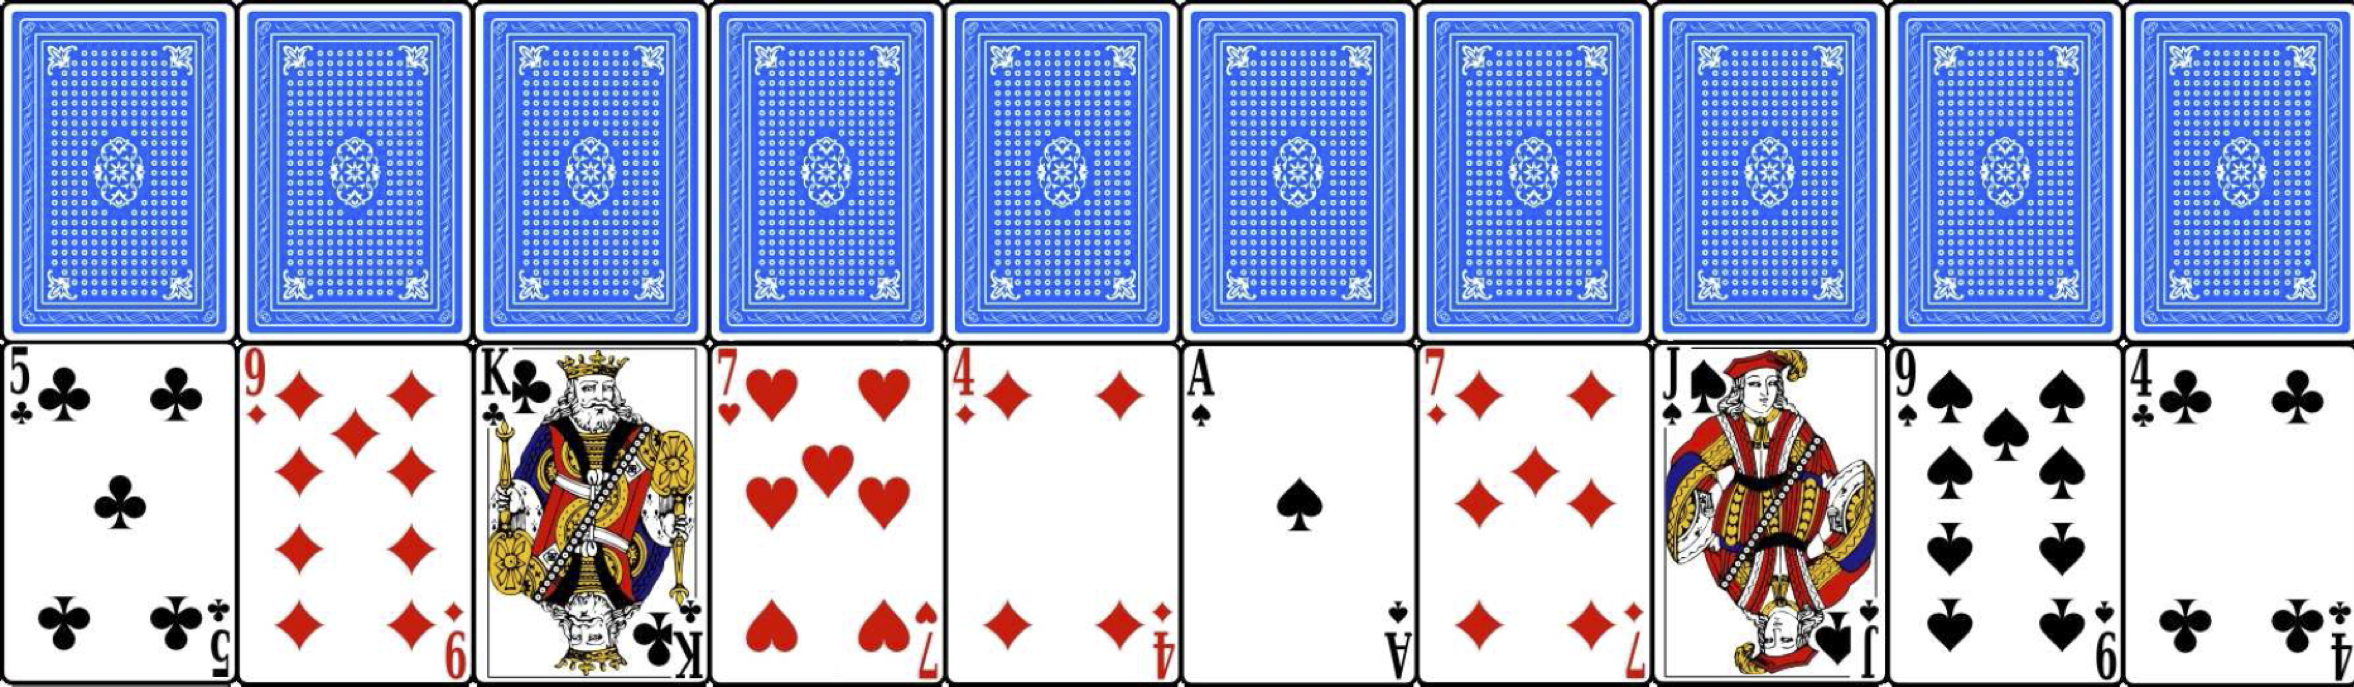
\includegraphics[width=0.7\textwidth]{cards.png}
        \end{center}

        \bigskip

        $H_0\colon$ испытуемый выбирает ответ наугад.

        $H_1\colon$ испытуемый может предсказывать цвета карт.

        Статистика $t$~--- число карт, цвета которых угаданы.

        $$P\left(t\geq9\left|H_0\right.\right)=11\cdot\frac1{2}^{10} = 0.0107421875,$$
        т.\,е. при $t=9$ получаем достигаемый уровень значимости $p \approx 0.01$~--- можно отклонять $H_0$.
    }

    \only<2>{
%%%%%%%%%%%%%%%%%%%%%%%%%%%%%%%%%%%%%%%%%%%%%%%%%%%%%%%%%%%%%%%%%%%%%%%
% В экспериментах Джозефа Райна процедуру отбора прошли 1000 человек. Девять из них угадали цвета 9 из 10 карт, еще двое угадали все 10 карт. Ни один из этих испытуемых в последующих экспериментах не подтвердил своих способностей, из чего Джозеф Райн сделал вывод, что экстрасенсам нельзя говорить о том, что они экстрасенсы, потому что от этого их способности сразу пропадают. Однако очевидно, что проблема кроется в чем-то другом.
% Если принять гипотезу о том, что экстрасенсов не существует, то вероятность того, что из тысячи человек хотя бы один случайно угадает цвета 9 или 10 из 10 карт, равна примерно 1.
% На рисунке показано, как описанная выше вероятность ведет себя в зависимости от количества испытуемых. Из графика видно, что она растет очень быстро. Уже при количестве испытуемых N = 100 вероятность найти хотя бы одного экстрасенса превышает 1/2. При N = 500 такая вероятность уже примерно равна единице.
% Тот факт, что с помощью этой статистической процедуры находятся экстрасенсы, является прекрасным примером влияния эффекта множественной проверки гипотез. При одновременной проверке большого количества гипотез вероятность совершить хотя бы одну ошибку первого рода (то есть ложно отвергнуть верную нулевую гипотезу) становится очень большой.
%%%%%%%%%%%%%%%%%%%%%%%%%%%%%%%%%%%%%%%%%%%%%%%%%%%%%%%%%%%%%%%%%%%%%%%
        Процедуру отбора прошли 1000 человек.

        Девять из них угадали цвета 9 из 10 карт, двое~--- цвета всех 10 карт.
        Ни~один в последующих экспериментах не подтвердил своих способностей.

        \bigskip

        Вероятность того, что из 1000 человек хотя бы один случайно угадает цвета 9 или 10 из 10 карт: $1-\left(1-11\cdot\frac1{2}^{10}\right)^{1000} \approx 0.9999796.$

        \bigskip

        \begin{center}
            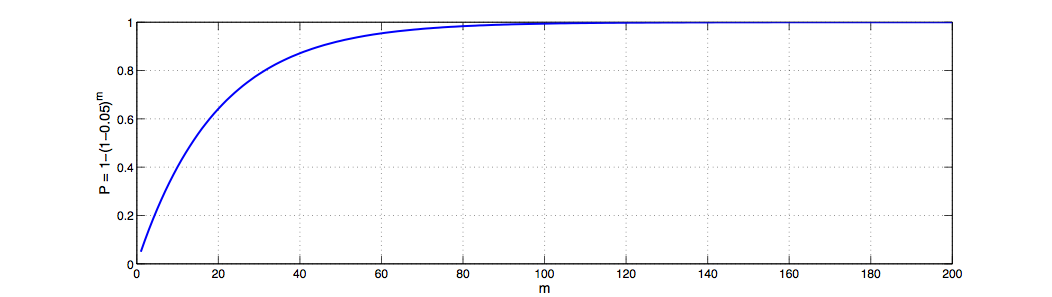
\includegraphics[width=0.85\textwidth,trim=33mm 0mm 30mm 7mm,clip]{prob_FWER.png}
        \end{center}
    }
\end{frame}


\begin{frame}{Случайные поля}

%%%%%%%%%%%%%%%%%%%%%%%%%%%%%%%%%%%%%%%%%%%%%%%%%%%%%%%%%%%%%%%%%%%%%%%
% Еще один яркий пример действия эффекта множественной проверки гипотез можно найти в нейронауке.
% Анализируются данные позитронно-эмиссионной томографии или функциональной магнитно-резонансной томографии. Типичный дизайн такого эксперимента следующий: берётся контрольная группа испытуемых, с которыми ничего не происходит, и измеряется активность их мозга. Затем те же измерения производят с другой группой испытуемых, состояние которых каким-то образом изменили. Далее эти две выборки сравнивают, пытаясь выяснить, на какие области мозга подействовало различие между двумя экспериментальными условиями.
% Решение такой задачи связано с проверкой очень большого количества гипотез. Фактически для двумерного изображения мозга гипотеза проверяется в каждой точке, для трехмерного изображения мозга, которое возникает при магнитно-резонансной томографии, гипотеза проверяется в каждом вокселе (то есть в каждом трехмерном пикселе трехмерного изображения мозга). Пикселей могут быть тысячи, вокселей могут быть миллионы. Таким образом, требуется проверить очень много гипотез. И если ничего не делать, эффект множественной проверки гипотез будет проявляться очень ярко.
%%%%%%%%%%%%%%%%%%%%%%%%%%%%%%%%%%%%%%%%%%%%%%%%%%%%%%%%%%%%%%%%%%%%%%%
    \begin{center}
        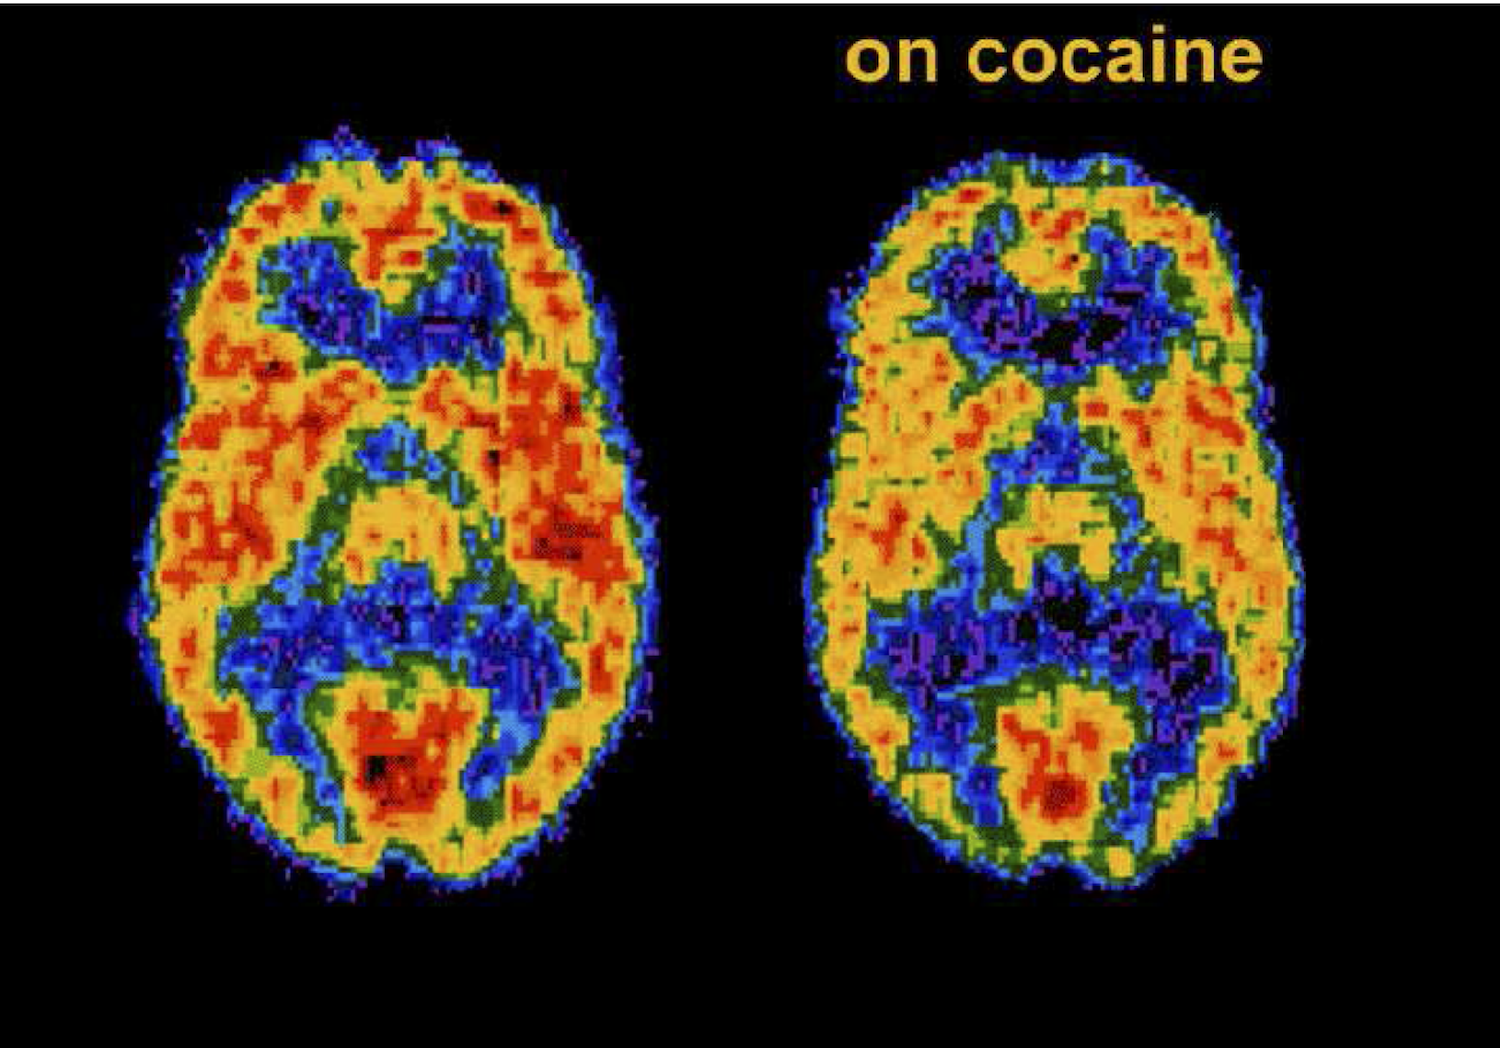
\includegraphics[width=0.6\textwidth]{cocaine.png}
    \end{center}
	
\end{frame}
\begin{frame}{Лосось (бывший)}
%%%%%%%%%%%%%%%%%%%%%%%%%%%%%%%%%%%%%%%%%%%%%%%%%%%%%%%%%%%%%%%%%%%%%%%
% Лучше всего это демонстрирует следующий пример. Команда исследователей воспроизвела один из типичных дизайнов нейронаучных экспериментов, в котором испытуемому последовательно и много раз демонстрируются похожие стимулы, затем активность его мозга в ответ на эти стимулы сравнивается с активностью его мозга в состоянии покоя. Роль испытуемого в этом эксперименте играл мертвый лосось. В качестве стимула ему показывали картинки с изображениями людей в различных социальных ситуациях. Как видно из рисунка, задача поиска областей, которые реагируют на этот стимул, была решена успешно. В мозге лосося были выявлены области, в которых активность значимо изменилась, они на рисунке обозначены красным.
% За последнее десятилетие методы анализа данных в нейронауке, в том числе методы поправки на множественную проверку гипотез, существенно улучшились. Поправка делается с привлечением теории гауссовых случайных полей и некоторых фактов из топологии. Это сложные и интересные методы, найти их можно по клчевому слову SPM - statistical parametrical mapping.
%%%%%%%%%%%%%%%%%%%%%%%%%%%%%%%%%%%%%%%%%%%%%%%%%%%%%%%%%%%%%%%%%%%%%%%
    \begin{center}
        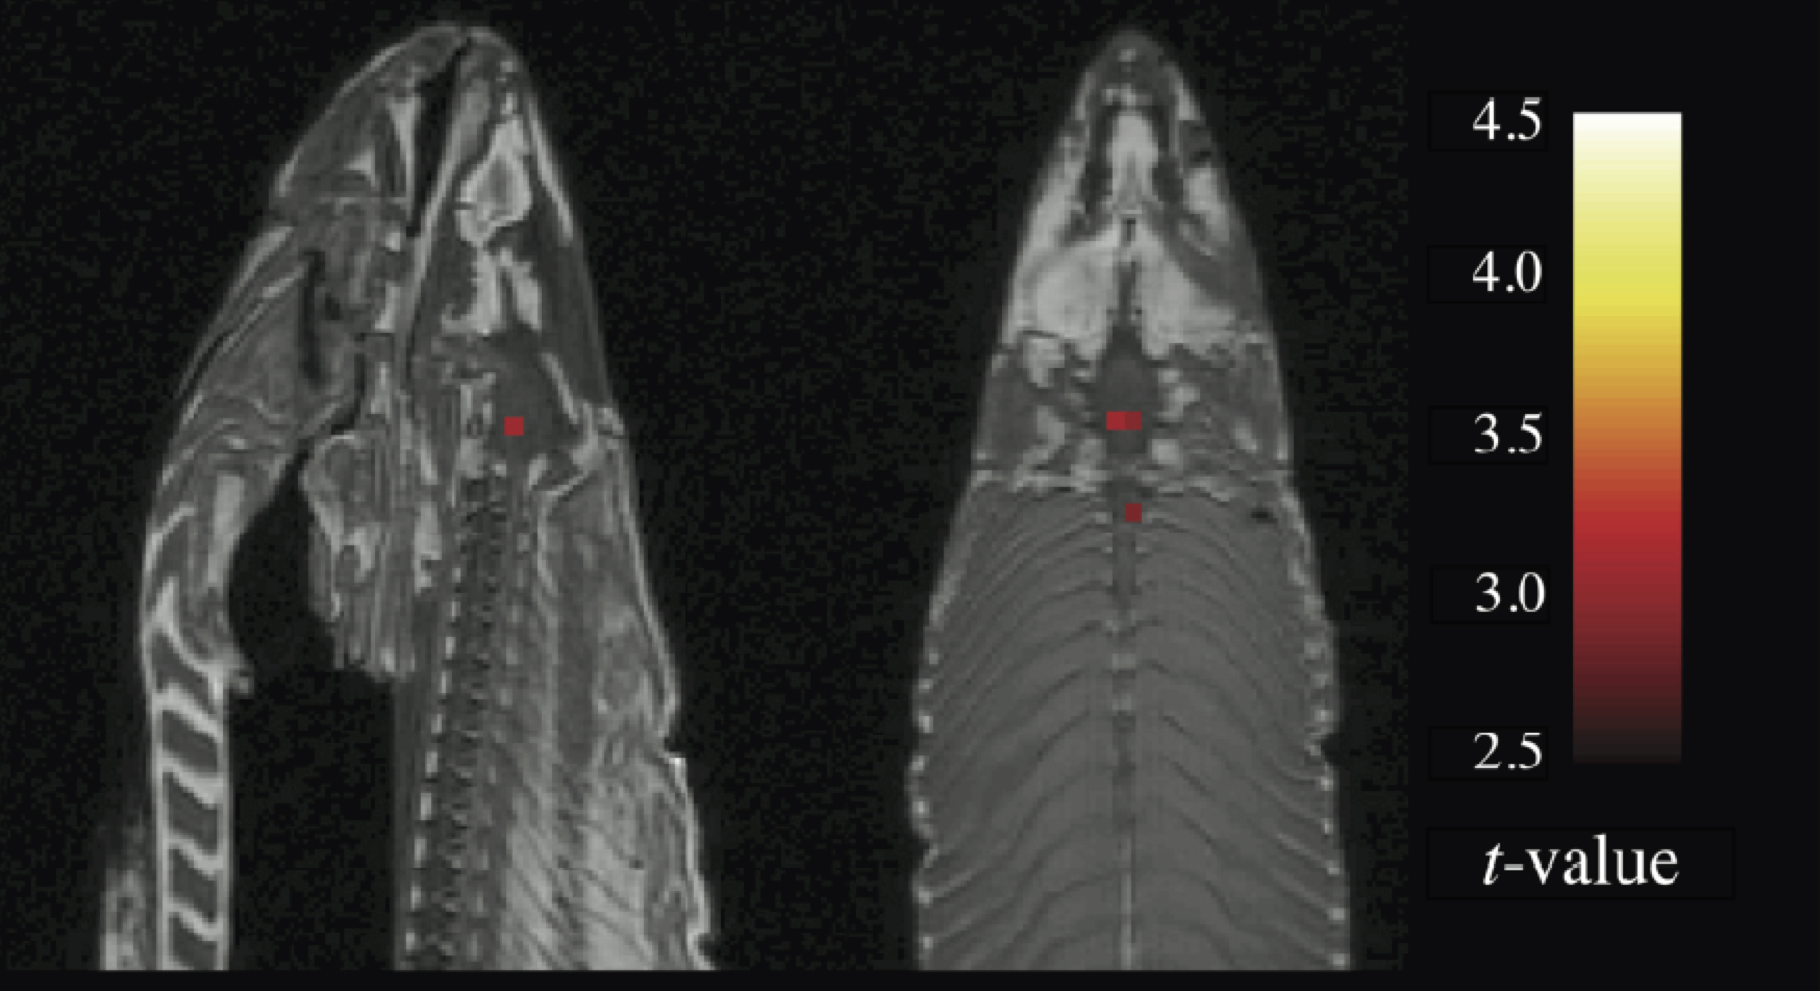
\includegraphics[width=0.8\textwidth]{salmon.png}
    \end{center}
\end{frame}

\section{Постановка задачи}
\subsection{Классическая схема проверки гипотез}
\begin{frame}{Математическая формулировка}
%%%%%%%%%%%%%%%%%%%%%%%%%%%%%%%%%%%%%%%%%%%%%%%%%%%%%%%%%%%%%%%%%%%%%%%
% В этой части будет дана математическая постановка задачи множественной проверки гипотез. Для этого полезно вспомнить, как ставится задача однократной проверки гипотез.
% Имеется некоторая выборка X объема n из неизвестного распределения P. Проверяется нулевая гипотеза H0 о распределении P против общей альтернативы H1. Это делается с помощью статистики T, которая является функцией от выборки. Для этой статистики известно нулевое распределение F (x), то есть распределение при справедливости нулевой гипотезы. По этому нулевому распределению, по его хвостам (разным, в зависимости от типа альтернативы) вычисляется достигаемый уровень значимости, то есть вероятность получить такое же значение статистики, какое было получено в эксперименте, или ещё более экстремальное. Достигаемый уровень значимости сравнивается с порогом альфа — уровнем значимости (типичное значение 0.05). Если достигаемый уровень значимости меньше, чем альфа, то нулевая гипотеза отвергается в пользу альтернативы.
		\begin{center}
	\vspace{-10pt}
	\begin{tabular}{rl}
		выборка:                        & $X^n=\left(X_1,\ldots,X_n\right), \; X \sim \prob \in \Omega$         \\
		нулевая гипотеза:               & $H_0\colon \prob\in\omega, \;\; \omega\in\Omega$ \\
		альтернатива:                   & $H_1\colon \prob\notin\omega$ \\
		статистика:                     & $T\left(X^n\right), \;\; T\left(X^n\right)\sim F\left(x\right) \;\text{при}\; \prob\in\omega$ \\
		& \;\;\;\;\;\;\;\;\;\;\;\;\;\; $T\left(X^n\right)\not\sim F\left(x\right) \;\text{при}\; \prob\notin\omega$ \\
		\multicolumn{2}{c}{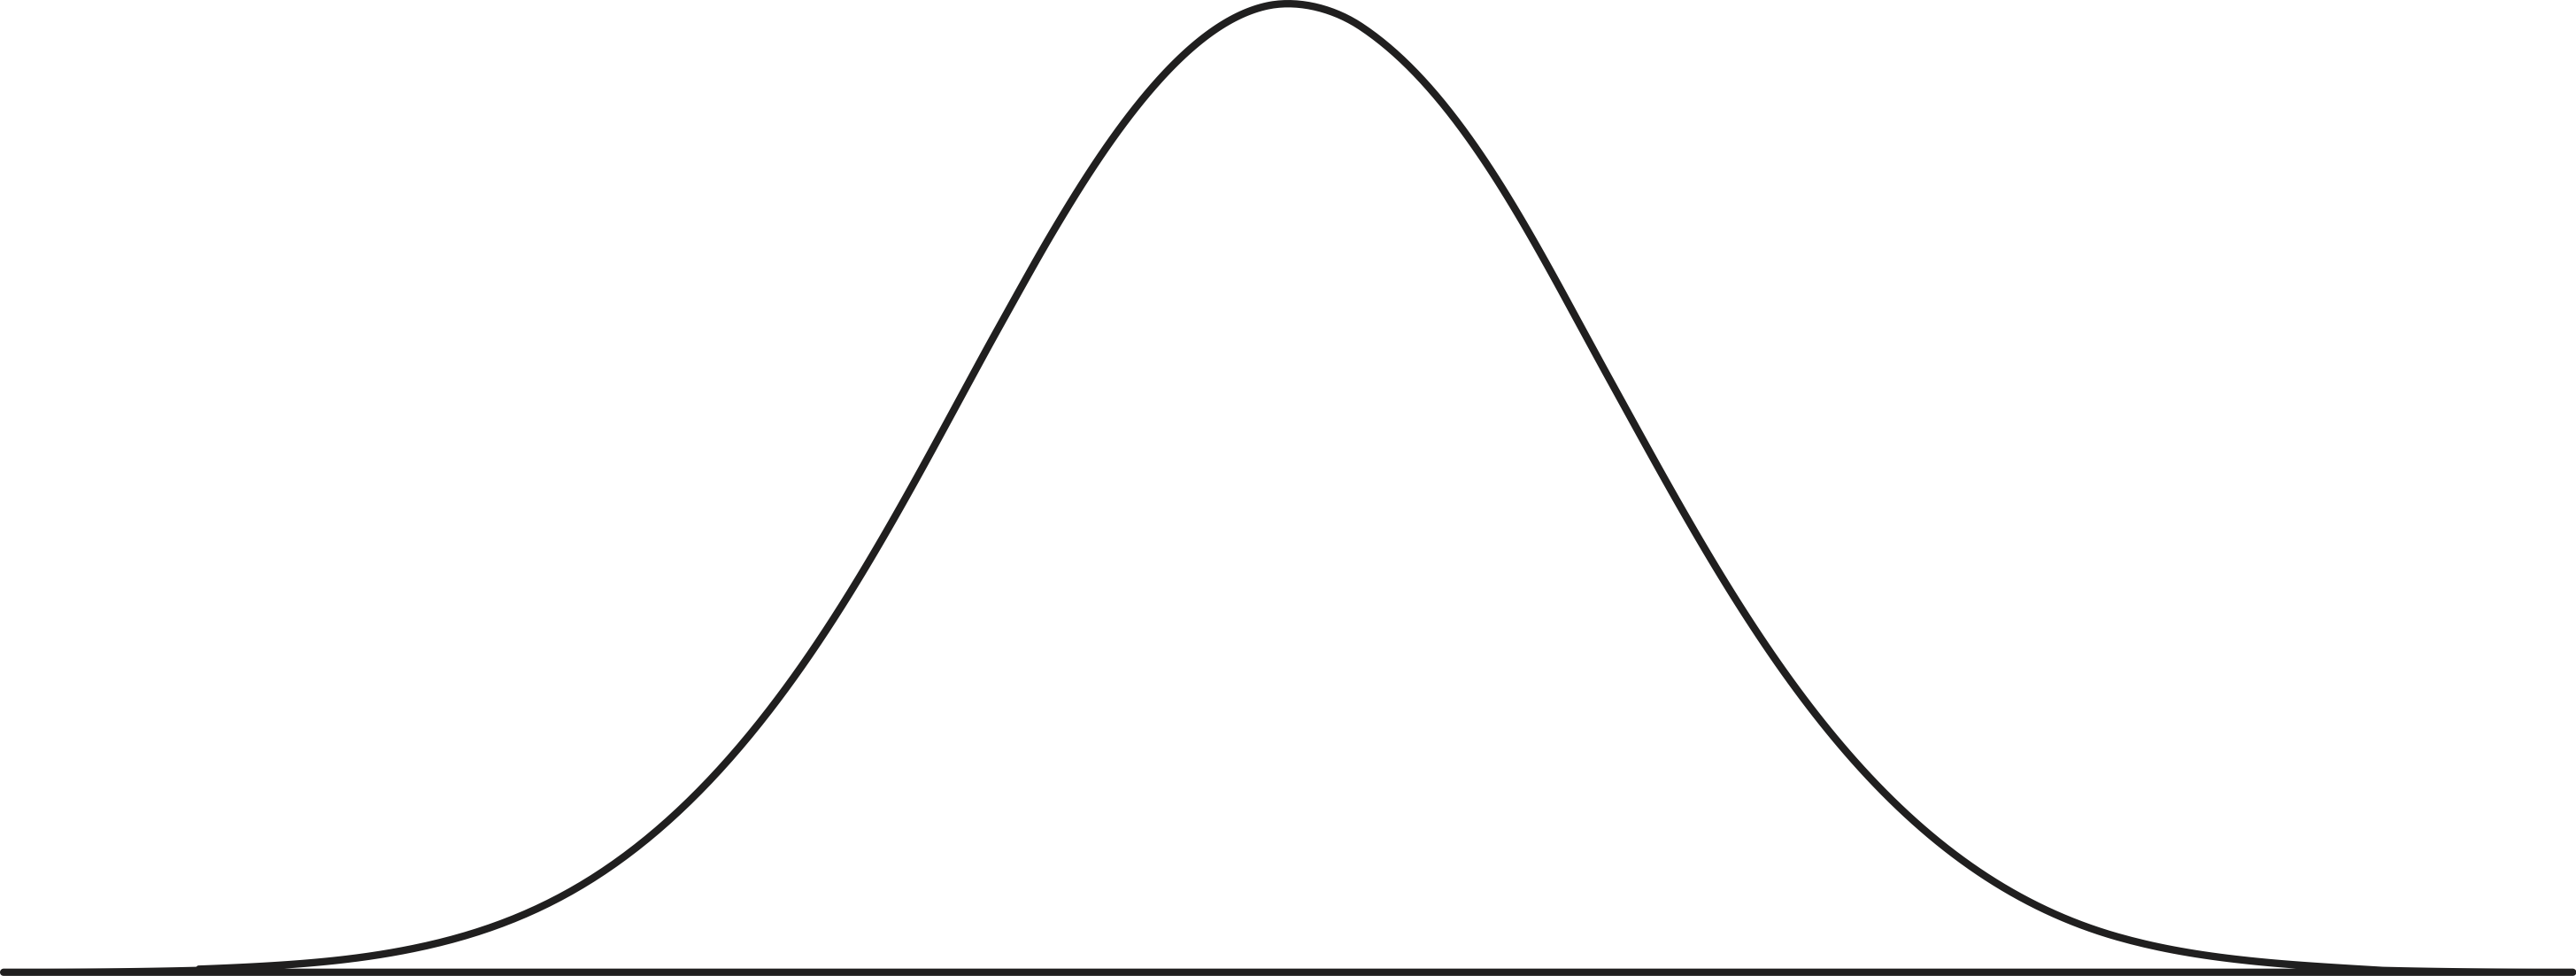
\includegraphics[width=0.2\textwidth]{stats1.png}} \\
		реализация выборки:             & $x^n=\left(x_1,\ldots,x_n\right)$ \\
		реализация статистики:          & $t = T \left(x^n\right)$ \\
		достигаемый уровень значимости: & $p\left(x^n\right)$~--- вероятность при $H_0$ получить \\
		& $T \left(X^n\right)=t$ или ещё более экстремальное\\
		\multicolumn{2}{c}{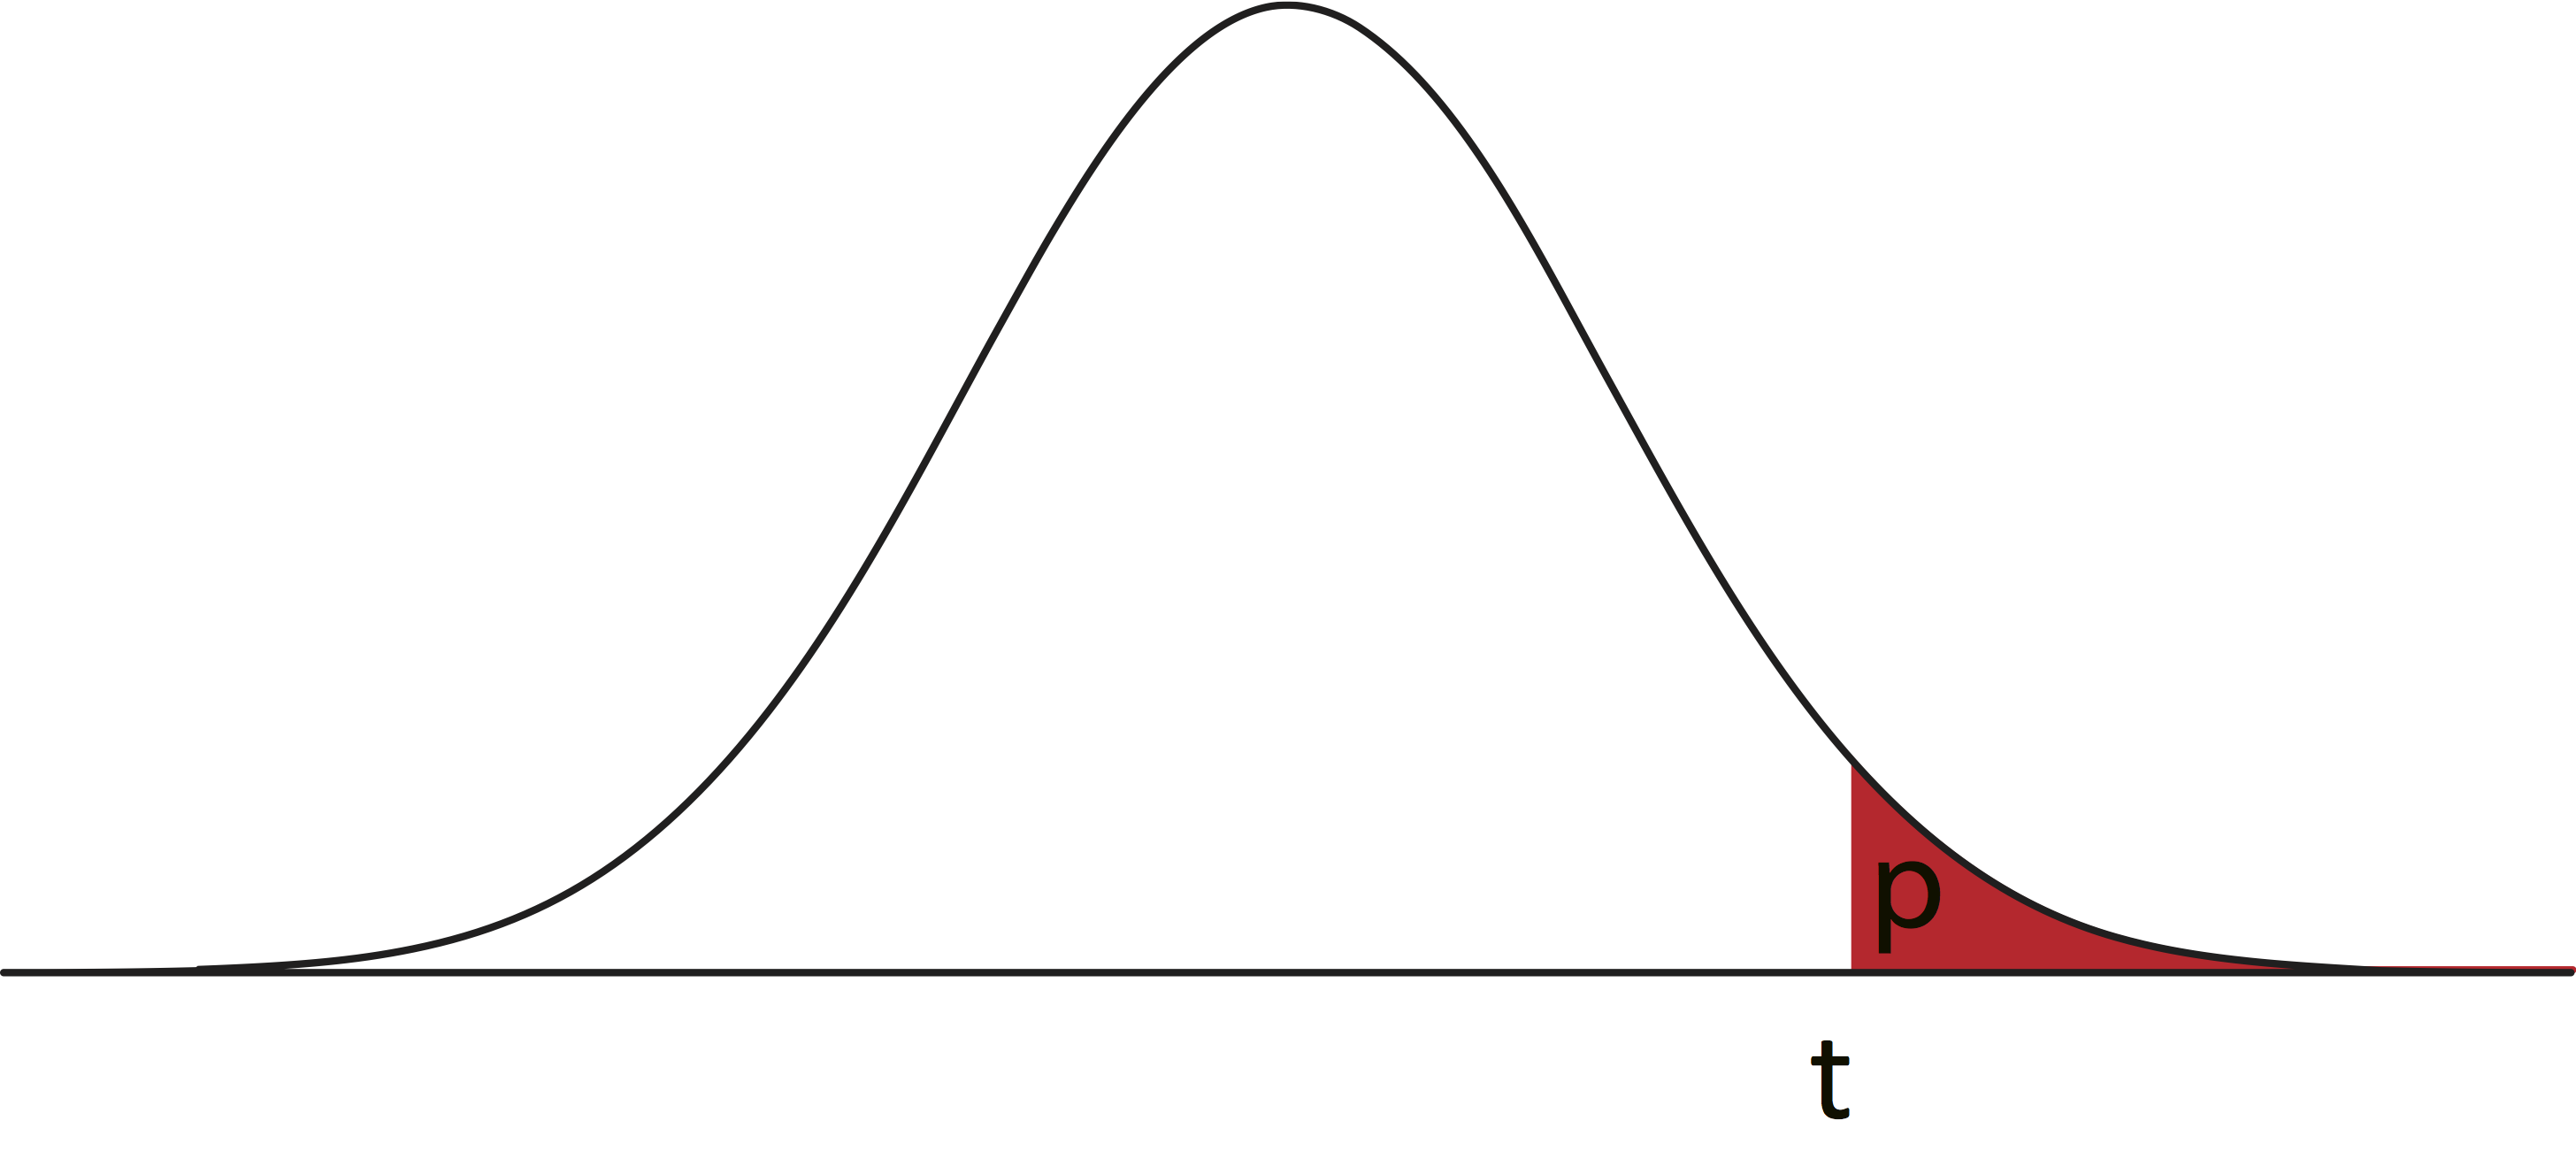
\includegraphics[width=0.2\textwidth]{stats2.png}} \\
		\multicolumn{2}{c}{ $p\left(x^n\right) = \prob\left(T\geq t\left|H_0\right.\right)$ } \\
		\multicolumn{2}{c}{Гипотеза отвергается при $p\left(x^n\right)\leq\alpha,\;\;\alpha$~--- уровень значимости} \\
	\end{tabular}
\end{center}
\end{frame}

\begin{frame}{Правило проверки гипотезы}
    \vspace{-3pt}
    \begin{center}
     	\includegraphics[height=0.85\textheight]{rememberkids.png}
    \end{center}
\end{frame}

\begin{frame}{Несимметричность задачи проверки гипотезы}
%%%%%%%%%%%%%%%%%%%%%%%%%%%%%%%%%%%%%%%%%%%%%%%%%%%%%%%%%%%%%%%%%%%%%%%
% При однократной проверке гипотезы всегда есть вероятность совершить ошибку первого или второго рода. Механизм проверки гипотез построен так, что вероятность ошибки первого рода, то есть вероятность ложно отвергнуть верную нулевую гипотезу, сверху ограничена достигаемым уровнем значимости альфа
%%%%%%%%%%%%%%%%%%%%%%%%%%%%%%%%%%%%%%%%%%%%%%%%%%%%%%%%%%%%%%%%%%%%%%%

    \begin{center}
        \begin{tabular}{ |r | c | c | }
        \hline
                          & $H_0$ верна         & $H_0$ неверна \\ \hline
        $H_0$ принимается & $H_0$ верно принята & Ошибка второго рода \\ \hline
        $H_0$ отвергается & Ошибка первого рода & $H_0$ верно отвергнута\\
        \hline
        \end{tabular}
    \end{center}

    \bigskip

    Вероятность ошибки первого рода жёстко ограничивается малой величиной:
    $$p = P\left(T\left(X^n\right)\geq t \left|H_0\right.\right) = P\left(p\leq\alpha\left|H_0\right.\right) \leq \alpha.$$

    \bigskip

    Вероятность ошибки второго рода минимизируется путём выбора достаточно мощного критерия.
\end{frame}

\subsection{Математическая постановка}
\begin{frame}{Математическая постановка}
%%%%%%%%%%%%%%%%%%%%%%%%%%%%%%%%%%%%%%%%%%%%%%%%%%%%%%%%%%%%%%%%%%%%%%%
% Теперь можно разобраться с постановкой задачи множественной проверки гипотез (таблица 9.3). Пусть имеется m выборок, каждая своего размера, и из своего распределения. Каждой выборке соответствует своя гипотеза нулевая гипотеза Hi и альтернатива Hi'. Каждая из гипотез проверяется своей статистикой Ti. Для каждой из статистик известно свое нулевое распределение. Таким образом, можно вычислить достигаемые уровни значимости всех гипотез. 
% Пусть M — это множество индексов 1, ..., m, M0 — это множество индексов верных нулевых гипотез, пусть его мощность равна m0. Естественно, это множество неизвестно, потому что иначе не было бы смысла проверять гипотезы. Пусть R — это множество индексов отвергаемых гипотез, а его мощность равна R. Тогда пересечение множеств R и M0 состоит из неверно отвергнутых гипотез. Мощность этого множества обозначается V , это есть число ошибок первого рода.
% По аналогии с задачей однократной проверки гипотез можно составить таблицу 2x2, в которой будет стоят количество верных и неверных, принятых и отвергнутых гипотез. Из всех величин, записанных в таблице, известна только m — общее число гипотез. А единственный параметр, которым можно управлять, — это R, количество отвергаемых гипотез. При этом самая пугающая величина — это V , количество ошибок первого рода. Хочется совершать мало ошибок первого рода, но при этом единственное, что можно делать, — это перераспределять по этой таблице гипотезы из второй строки в первую. То есть, чтобы совершать мало ошибок первого рода, нужно отвергать меньше гипотез.
% Задача множественной проверки гипотез поставлена, теперь нужно её решить. Интерес представляет некоторая статистическая процедура, которая дает гарантии на значение V, оно не должно быть слишком большим.
%%%%%%%%%%%%%%%%%%%%%%%%%%%%%%%%%%%%%%%%%%%%%%%%%%%%%%%%%%%%%%%%%%%%%%%
    \vspace{-10pt}
    \begin{center}
        \begin{tabular}{ r l }
                данные:                        & $\mathbf{X}=\{X_1^{n_1},\ldots,X_m^{n_m}\}, \;\; X_i \sim P_i \in \Omega_i$         \\
                нулевые гипотезы:              & $H_i\colon P_i\in\omega_i, \;\; \omega_i\in\Omega_i$ \\
                альтернативы:                  & $H'_i\colon P_i\notin\omega_i$ \\
                статистики:                    & $T_i=T\left(X_i^{n_i}\right)$ проверяет $H_i$ против $H'_i$ \\
                реализации статистик:          & $t_i=T\left(x_i^{n_i}\right)$ \\
                достигаемые уровни значимости: & $p_i=p\left(x_i^{n_i}\right), \;\; i=1,\ldots,m$
        \end{tabular}
    \end{center}

    \bigskip

    $\mathbf{M}=\left\{1,2,\ldots,m\right\}$

    $\mathbf{M_0} = \mathbf{M_0}\left(P\right) = \left\{i\colon H_i~\text{верна}\right\}$ "--- индексы верных гипотез, $\left|\mathbf{M_0}\right|=m_0$

    $\mathbf{R} = \mathbf{R}\left(P,\alpha\right) = \left\{i\colon H_i~\text{отвергнута}\right\}$ "--- индексы отвергаемых гипотез, $\left|\mathbf{R}\right|=R$

    $V=\left|\mathbf{M_0}\cap\mathbf{R}\right|$ "--- число ошибок первого рода
    \begin{center}
        \begin{tabular}{ |r | c | c | c |}
        \hline
                                & Число верных $H_i$ & Число неверных $H_i$ & Всего \\ \hline
        Число принятых $H_i$    & $U$                & $T$                  & $m-R$\\ \hline
        Число отвергнутых $H_i$ & $V$                & $S$                  & $R$\\ \hline
        Всего                   & $m_0$              & $m-m_0$              & $m$\\
        \hline
        \end{tabular}
    \end{center}
\end{frame}


\section{FWER}
\subsection{FWER}
\begin{frame}{Многомерные обобщения ошибки первого рода}
%%%%%%%%%%%%%%%%%%%%%%%%%%%%%%%%%%%%%%%%%%%%%%%%%%%%%%%%%%%%%%%%%%%%%%%
% Напрямую с V работать не очень удобно, поэтому, как правило, берут некоторые меры, определенные над V , и работают с ними. Одна из самых распространенных таких мер — это групповая вероятность ошибки первого рода (familywise error rate). По определению это вероятность совершить хотя бы одну ошибку первого рода. Эту величину хочется контролировать на уровне альфа. То есть, хочется построить такую статистическую процедуру, что вероятность совершить хотя бы одну ошибку первого рода будет не больше, чем альфа. Возникает вопрос, как этого добиться.
% Единственный имеющийся в распоряжении инструмент — это уровни значимости альфа1 , . . . , альфаm , на которых проверяются гипотезы H1, . . . , Hm. Никаких других параметров в проверке гипотез нет. Ставится задача выбрать эти уровни так, чтобы обеспечить ограничение FWER ? альфа
%%%%%%%%%%%%%%%%%%%%%%%%%%%%%%%%%%%%%%%%%%%%%%%%%%%%%%%%%%%%%%%%%%%%%%%
    \textbf{Групповая вероятность ошибки} первого рода (familywise error rate):
    $$\FWER = P\left(V>0\right).$$

    \bigskip

    Контроль над групповой вероятностью ошибки на уровне $\alpha$ означает $$\FWER = P \left( V >0 \right) \leq \alpha ~~\forall P.$$

    \bigskip

    Как этого добиться?

    Параметры $\alpha_1,\ldots,\alpha_m$~--- уровни значимости, на которых необходимо проверять гипотезы $H_1,\ldots,H_m;$ задача~--- выбрать их так, чтобы обеспечить $\FWER\leq\alpha.$
\end{frame}

\subsection{Одношаговые методы}
\begin{frame}{Поправка Бонферрони}
    \only<1>{
%%%%%%%%%%%%%%%%%%%%%%%%%%%%%%%%%%%%%%%%%%%%%%%%%%%%%%%%%%%%%%%%%%%%%%%
% Самый простой способ решить поставленную выше задачу — это использовать поправку Бонферрони. В методе Бонферрони достигаемые уровни значимости всех гипотез сравниваются с величиной alpha/m :
% Альтернативный способ — преобразовать все достигаемые уровни значимости (p-value): p ?i =min(1,mpi). Эти модифицированные достигаемые уровни значимости и будут сравниваться с исходным порогом альфа: Hi отвергается при p ?i ? alpha. При такой процедуре точно так же контролируется величина FWER, как и при изменении порога.
% Легко показать, что метод Бонферрони контролирует групповую вероятность ошибки первого рода на уровне alpha. Это будет единственная теорема в курсе.
% Доказательство По определению Familywise error rate (FWER) — это вероятность совершить хотя бы одну ошибку первого рода; Вероятность объединения событий можно оценить сверху через сумму вероятностей этих событий по неравенству Буля; Далее можно воспользоваться свойством достигаемого уровня значимости; m0 < m, следовательно Исходное утверждение доказано.
%%%%%%%%%%%%%%%%%%%%%%%%%%%%%%%%%%%%%%%%%%%%%%%%%%%%%%%%%%%%%%%%%%%%%%%
    \textbf{Метод Бонферрони}: $$\alpha_1=\ldots=\alpha_m=\alpha/m.$$

    \begin{Th}\label{Bonf}
        Если гипотезы $H_i, \;\; i=1,\ldots,m,$ отвергаются при $p_i\leq \alpha / m,$ то $\FWER\leq\alpha.$
    \end{Th}
    
    \vspace{-5pt}
    
    \begin{proof}
        $$\FWER  =  P\left(V>0\right)  =  P\left(\bigcup_{i=1}^{m_0} \left\{ p_i \leq \alpha / m \right\} \right)  \leq  \sum_{i=1}^{m_0}P\left( p_i \leq \alpha / m \right) \leq$$
        $$\leq  \sum_{i=1}^{m_0} \alpha/m  =  \frac{m_0}{m}\alpha  \leq  \alpha.$$
    \end{proof}

    Альтернативный вид~--- переход к модифицированным достигаемым уровням значимости:
    $$\tilde{p}_i = \min\left(1,mp_i\right).$$
    }

    \only<2>{
%%%%%%%%%%%%%%%%%%%%%%%%%%%%%%%%%%%%%%%%%%%%%%%%%%%%%%%%%%%%%%%%%%%%%%%
% Те, кто когда-нибудь сталкивались с неравенством Буля, знают, что оценка вероятности объединения событий через сумму вероятностей этих событий очень завышенная. Действительно, чтобы получить в этом месте доказательства точное равенство, нужно вычесть вероятности всех возможных пересечений. Цепочка неравенств в доказательстве теоремы показывает, что при использовании метода Бонферрони FWER не просто меньше, чем альфа, а намного меньше, чем альфа. В идеале хочется, чтобы вероятность совершить хотя бы одну ошибку первого рода была в точности равна альфа. При использовании метода Бонферрони эта вероятность ограничивается гораздо более низкой величиной, чем альфа. Это плохо, потому что перестраховываясь в отношении ошибки первого рода, мы неизбежно совершаем больше ошибок второго рода, то есть мощность такой статистической процедуры снижается.
%%%%%%%%%%%%%%%%%%%%%%%%%%%%%%%%%%%%%%%%%%%%%%%%%%%%%%%%%%%%%%%%%%%%%%%
    При увеличении $m$ в результате применения поправки Бонферрони мощность статистической процедуры резко уменьшается~--- шансы отклонить неверные гипотезы падают.

    \bigskip

    Пример: критерий Стьюдента для независимых выборок, 
    
    $X_1^n, X_1 \sim N\left(\mu_1,1\right),$ \;$X_2^n, X_2 \sim N\left(\mu_2,1\right),$ \; $\mu_1-\mu_2=1,$
    
    $H_0\colon \mathbb{E}X_{1}=\mathbb{E}X_{2},$ \; $H_1\colon \mathbb{E}X_{1}\neq\mathbb{E}X_{2}.$         

    \bigskip

    \begin{center}
        \begin{tabular}{ |c|c|c|}
            \hline
            $m$  & $n$ & Мощность \\\hline
            1    & 23  & 0.9 \\\hline
            10   & 23  & 0.67 \\\hline
            100  & 23  & 0.37 \\\hline
            1000 & 23  & 0.16 \\\hline
            1000 & 62  & 0.9 \\\hline
        \end{tabular}
    \end{center}

    \bigskip

    Если проверяется одновременно 1000000~гипотез, при размере выборок $n=10$ мощность $0.9$ достигается при расстоянии между средними выборок в пять стандартных отклонений.
    }
\end{frame}

\begin{frame}{Модельный эксперимент}
%%%%%%%%%%%%%%%%%%%%%%%%%%%%%%%%%%%%%%%%%%%%%%%%%%%%%%%%%%%%%%%%%%%%%%%
% Возьмем 50 выборок из нормального распределения N (1, 1) и еще 150 — из стандартного нормального рас- пределения N (0, 1). Объём всех выборок n = 20. На каждой из этих выборок проверяется гипотеза о равенстве среднего 0 против двусторонней альтернативы с помощью критерия Стьюдента.
% Если не делать никакой поправки на множественную проверку, в результате получится таблица. Видно, что отвергнуты все 50 неверных гипотез, но, к сожалению, вместе с ними отвергнуты еще и 8 верных, то есть совершилось 8 ошибок первого рода.
% Если делать поправку методом Бонферрони, гипотезы из второй строчки предыдущей таблицы перераспределяются в первую, результат — следующая таблица. В этом случае ни одна верная нулевая гипотеза не отвергается, то есть нет ни одной ошибки первого рода. Но, к сожалению, вместе с этим исчезла возможность отвергнуть больше половины неверных нулевых гипотез: из 50 удалось отвергнуть только 23. То есть за гарантии в отношении ошибки первого рода пришлось отплатить тем, что найдено меньше неверных нулевых гипотез.
%%%%%%%%%%%%%%%%%%%%%%%%%%%%%%%%%%%%%%%%%%%%%%%%%%%%%%%%%%%%%%%%%%%%%%%
    $n = 20, \;\; m=200, \;\; m_0 = 150;$

    $X_i^n, X_{i} \sim N\left(0,1\right), \;i=1,\ldots,m_0;$

    $X_i^n, X_{i} \sim N\left(1,1\right), \;i=m_0+1,\ldots,m;$

    $H_i\colon \mathbb{E}X_{i} = 0, \;\; H_i'\colon \mathbb{E}X_{i} \neq 0.$

    Для проверки используем одновыборочный критерий Стьюдента.

    \bigskip

    Без поправок:
    \begin{center}
        \begin{tabular}{ |r | c | c | c |}
        \hline
                          & Верных $H_i$ & Неверных $H_i$ & Всего \\ \hline
        Принятых $H_i$    & 142          & 0              & 142   \\ \hline
        Отвергнутых $H_i$ & 8            & 50             & 58    \\ \hline
        Всего             & 150          & 50             & 200   \\ \hline
        \end{tabular}
    \end{center}

    \bigskip

    Бонферрони:
    \begin{center}
        \begin{tabular}{ |r | c | c | c |}
        \hline
                          & Верных $H_i$ & Неверных $H_i$ & Всего \\ \hline
        Принятых $H_i$    & 150          & 27             & 177   \\ \hline
        Отвергнутых $H_i$ & 0            & 23             & 23    \\ \hline
        Всего             & 150          & 50             & 200   \\ \hline
        \end{tabular}
    \end{center}
\end{frame}

\subsection{Нисходящие методы}
\begin{frame}{Нисходящие методы множественной проверки гипотез}
%%%%%%%%%%%%%%%%%%%%%%%%%%%%%%%%%%%%%%%%%%%%%%%%%%%%%%%%%%%%%%%%%%%%%%%
%В методе Бонферрони уровни значимости для всех гипотез выбираются одинаковыми. Оказывается, если значения ai брать не одинаковыми, а разными, можно достичь лучшего результата. Для того, чтобы это сделать, необходимо использовать нисходящую процедуру множественной проверки гипотез. В общем виде она выглядит так. Из достигаемых уровней значимости составляется вариационный ряд: а все гипотезы переобозначаются так, чтобы их номера соответствовали номерам достигаемых уровней значимости в этом вариационном ряду:
%Дальше нужно самый маленький достигаемый уровень значимости p(1) сравнить с уровнем значимости альфа1. Если p(1) ? альфа1, то принимаются все нулевые гипотезы H(1), H(2), . . . , H(m), и процесс останавливается. p(1) < альфа1, то отклоняется гипотеза H(1), и процедура продолжается. На втором шаге сравниваются p(2) и альфа2. Если p(2) ? альфа2, то принимаются все оставшиеся гипотезы H(2), H(3), . . . , H(m), и процедура завершается. Если нет — H(2) отвергается, процедура продолжается, и т.д.
%Так в общем виде выглядит нисходящая процедура множественной проверки гипотез. Процедура называ- ется нисходящей, несмотря на то что нулевые гипотезы перебираются по возрастанию. Это немного странно и может смущать, но идея заключается в том, что нулевые гипотезы отвергаются последовательно, начиная с наиболее значимых, то есть движение происходит по убыванию значимости.
%%%%%%%%%%%%%%%%%%%%%%%%%%%%%%%%%%%%%%%%%%%%%%%%%%%%%%%%%%%%%%%%%%%%%%%
    Составим вариационный ряд достигаемых уровней значимости: $$p_{(1)}\leq p_{(2)} \leq \ldots \leq p_{(m)},$$
    $H_{(1)}, H_{(2)}, \ldots, H_{(m)}$~--- соответствующие гипотезы.

    \bigskip

    \begin{enumerate}
    \item Если $p_{(1)}\geq\alpha_1,$ принять все нулевые гипотезы $H_{(1)}, H_{(2)}, \ldots, H_{(m)}$ и~остановиться; иначе отвергнуть $H_{(1)}$ и продолжить.
    \item Если $p_{(2)}\geq\alpha_2,$ принять все нулевые гипотезы $H_{(2)}, H_{(3)}, \ldots, H_{(m)}$ и~остановиться; иначе отвергнуть $H_{(2)}$ и продолжить.
    \item \ldots
    \end{enumerate}

    \bigskip

    Каждый достигаемый уровень значимости $p_{(i)}$ сравнивается со своим уровнем значимости $\alpha_i$.
\end{frame}

\begin{frame}{Метод Холма}
    \only<1>{
%%%%%%%%%%%%%%%%%%%%%%%%%%%%%%%%%%%%%%%%%%%%%%%%%%%%%%%%%%%%%%%%%%%%%%%а
% Метод Холма — это нисходящая процедура множественной проверки гипотез со следующими уровнями значимости
% Этот метод обеспечивает безусловный контроль над FWER. Это показать немного сложнее, чем для метода Бонферрони, поэтому доказательство здесь приведено не будет. Вместо того, чтобы сравнить исходные достигаемые уровни значимости с модифицированными альфаi, можно их модифицировать и сравнивать с исходным порогом альфа. Так выглядит формула для модифицированных достигаемых уровней значимости метода Холма:
%%%%%%%%%%%%%%%%%%%%%%%%%%%%%%%%%%%%%%%%%%%%%%%%%%%%%%%%%%%%%%%%%%%%%%%а
    \textbf{Метод Холма}~--- нисходящая процедура со следующими уровнями значимости:
    $$\alpha_1 = \frac{\alpha}{m}, \; \alpha_2 = \frac{\alpha}{m-1}, \; \ldots, \; \alpha_i = \frac{\alpha}{m-i+1}, \; \ldots, \; \alpha_m = \alpha.$$

    \bigskip

    Метод обеспечивает контроль над $\FWER$ на уровне $\alpha$ при любых $p_i$ и $T_i$.

    \bigskip

    Модифицированные достигаемые уровни значимости:
    $$\tilde{p}_{(i)} = \min\left(1, \max \left(\left(m-i+1\right)p_{(i)}, \tilde{p}_{(i-1)}\right)\right).$$
    }

    \only<2>{
%%%%%%%%%%%%%%%%%%%%%%%%%%%%%%%%%%%%%%%%%%%%%%%%%%%%%%%%%%%%%%%%%%%%%%%
% Метод Холма всегда мощнее, чем метод Бонферрони, то есть, он всегда отвергает не меньше гипотез, чем метод Бонферрони, потому что его уровни значимости всегда не меньше, чем из метода Бонферрони.
%%%%%%%%%%%%%%%%%%%%%%%%%%%%%%%%%%%%%%%%%%%%%%%%%%%%%%%%%%%%%%%%%%%%%%%
    Метод Холма равномерно мощнее поправки Бонферрони, поскольку все его уровни значимости $\alpha_i$ не меньше:
    \begin{center}
        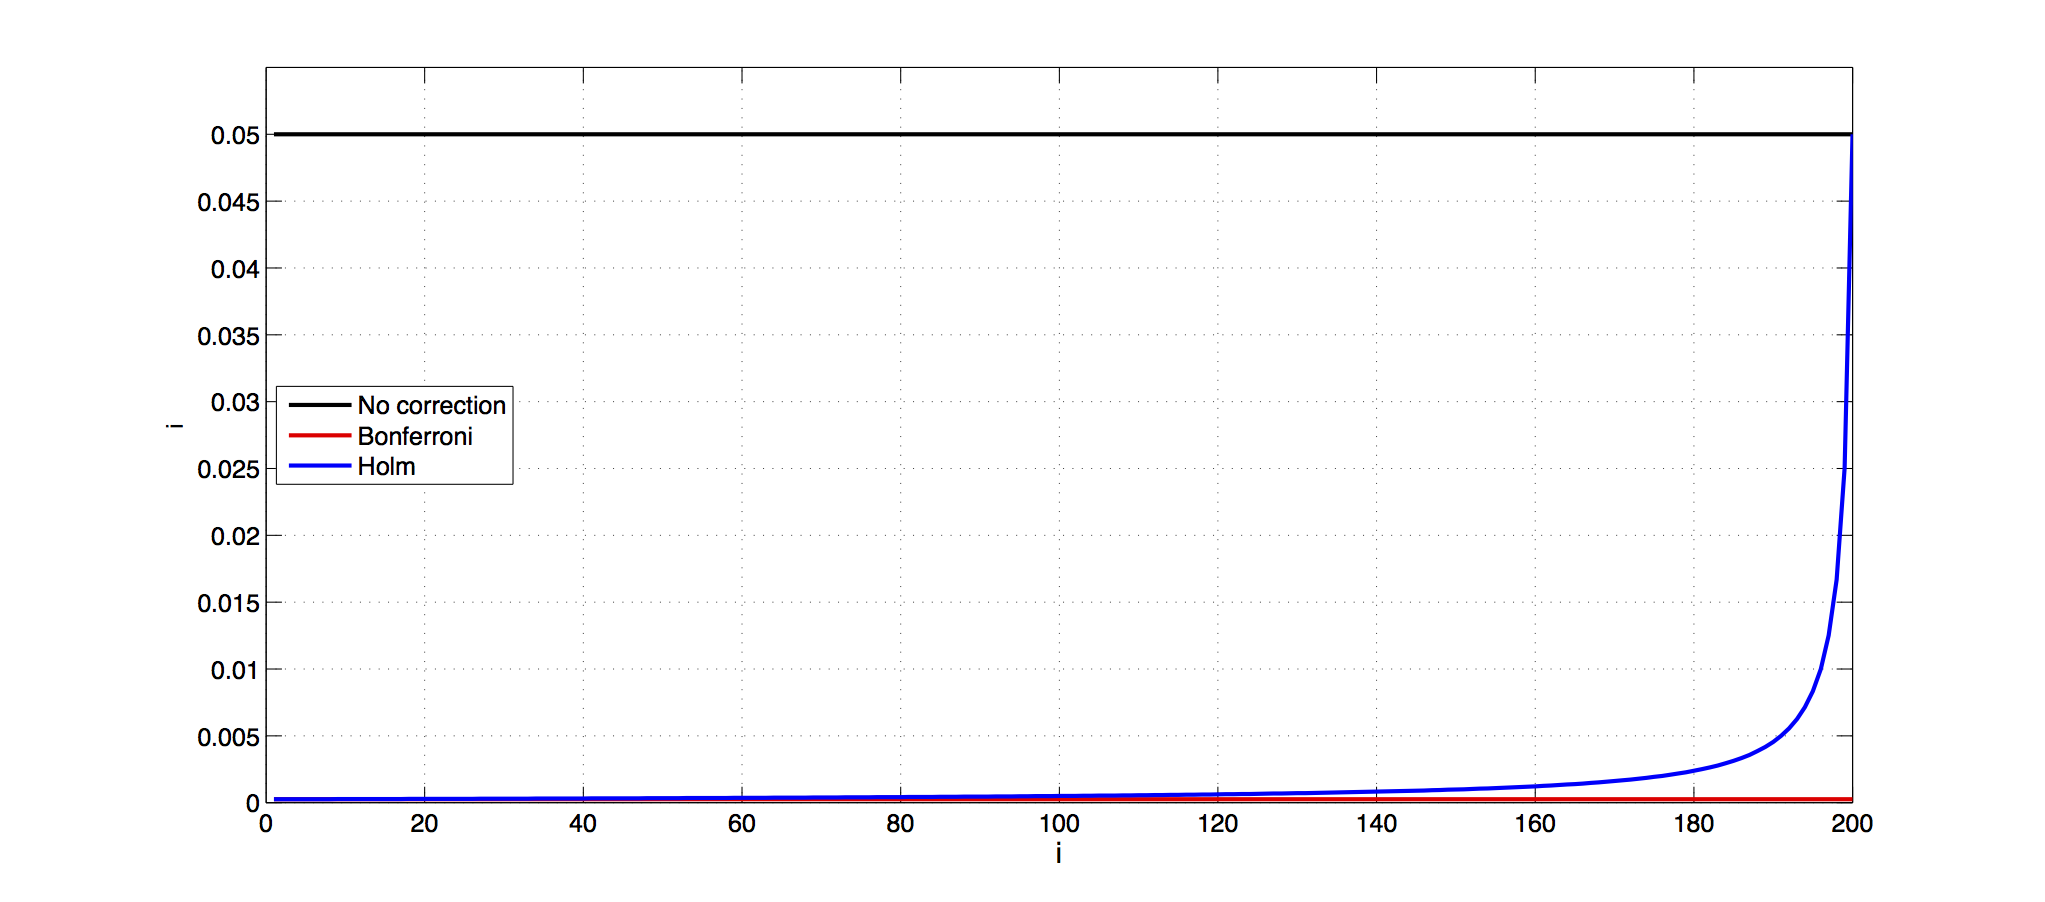
\includegraphics[width=0.85\textwidth]{alphas1.png}
    \end{center}

    }
\end{frame}

\begin{frame}{Модельный эксперимент}
    \only<1>{
%%%%%%%%%%%%%%%%%%%%%%%%%%%%%%%%%%%%%%%%%%%%%%%%%%%%%%%%%%%%%%%%%%%%%%%
%Для демонстрации работы метода Холма вернёмся к нашему модельному эксперименту.
%На графике показаны отсортированные достигаемые уровни значимости. По горизонтальной оси отложен номер в вариационном ряду, а по вертикальной оси — значения соответствующего достигаемого уровня значимости. Красные точки на графике — это неверные гипотезы, а синие точки — верные. Это типичный вид такого графика, на нём изображена как будто бы смесь двух треугольников: большого синего, соответствующего верным нулевым гипотезам, и маленького красного, соответствующего неверным. В месте соединения этих двух треугольников верные и неверные гипотеза смешиваются, и задача — где-то в этом месте правильно поставить порог, чтобы обеспечить теоретические гарантии на число ошибок первого рода.
%%%%%%%%%%%%%%%%%%%%%%%%%%%%%%%%%%%%%%%%%%%%%%%%%%%%%%%%%%%%%%%%%%%%%%%
    Отсортированные достигаемые уровни значимости:
    \begin{center}
        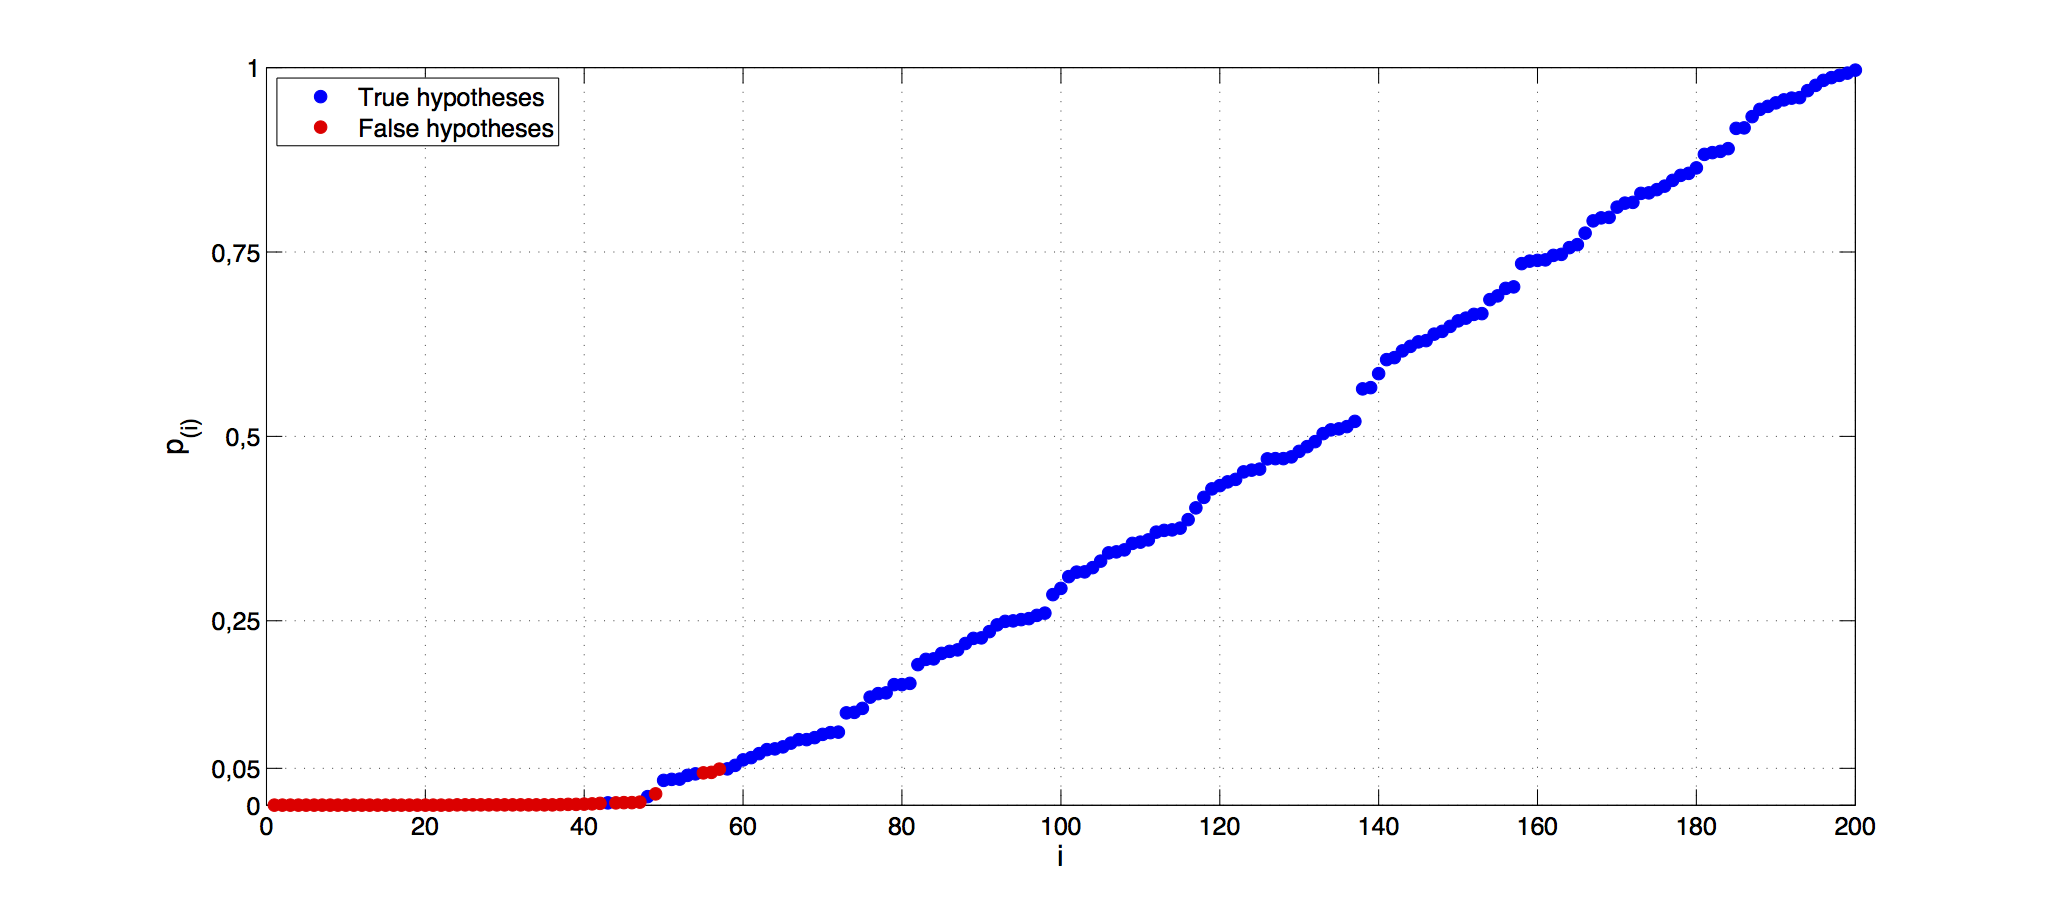
\includegraphics[width=0.8\textwidth]{ps_sort.png}
    \end{center}
        \begin{center}
        \begin{tabular}{ |r | c | c | c |}
        \hline
                          & Верных $H_i$ & Неверных $H_i$ & Всего \\ \hline
        Принятых $H_i$    & 142          & 0              & 142   \\ \hline
        Отвергнутых $H_i$ & 8            & 50             & 58    \\ \hline
        Всего             & 150          & 50             & 200   \\ \hline
        \end{tabular}
    \end{center}


    }

    \only<2>{
%%%%%%%%%%%%%%%%%%%%%%%%%%%%%%%%%%%%%%%%%%%%%%%%%%%%%%%%%%%%%%%%%%%%%%%
% На рисунке показаны модифицированные достигаемые уровни значимости, отсортированные по неубыванию, при использовании поправки Бонферрони. Результаты были приведены в таблице. Отвергаются 23 неверные нулевые гипотезы из 50 и ни одной верной.
%%%%%%%%%%%%%%%%%%%%%%%%%%%%%%%%%%%%%%%%%%%%%%%%%%%%%%%%%%%%%%%%%%%%%%%
    Модифицированные достигаемые уровни значимости, метод Бонферрони:
    \begin{center}
        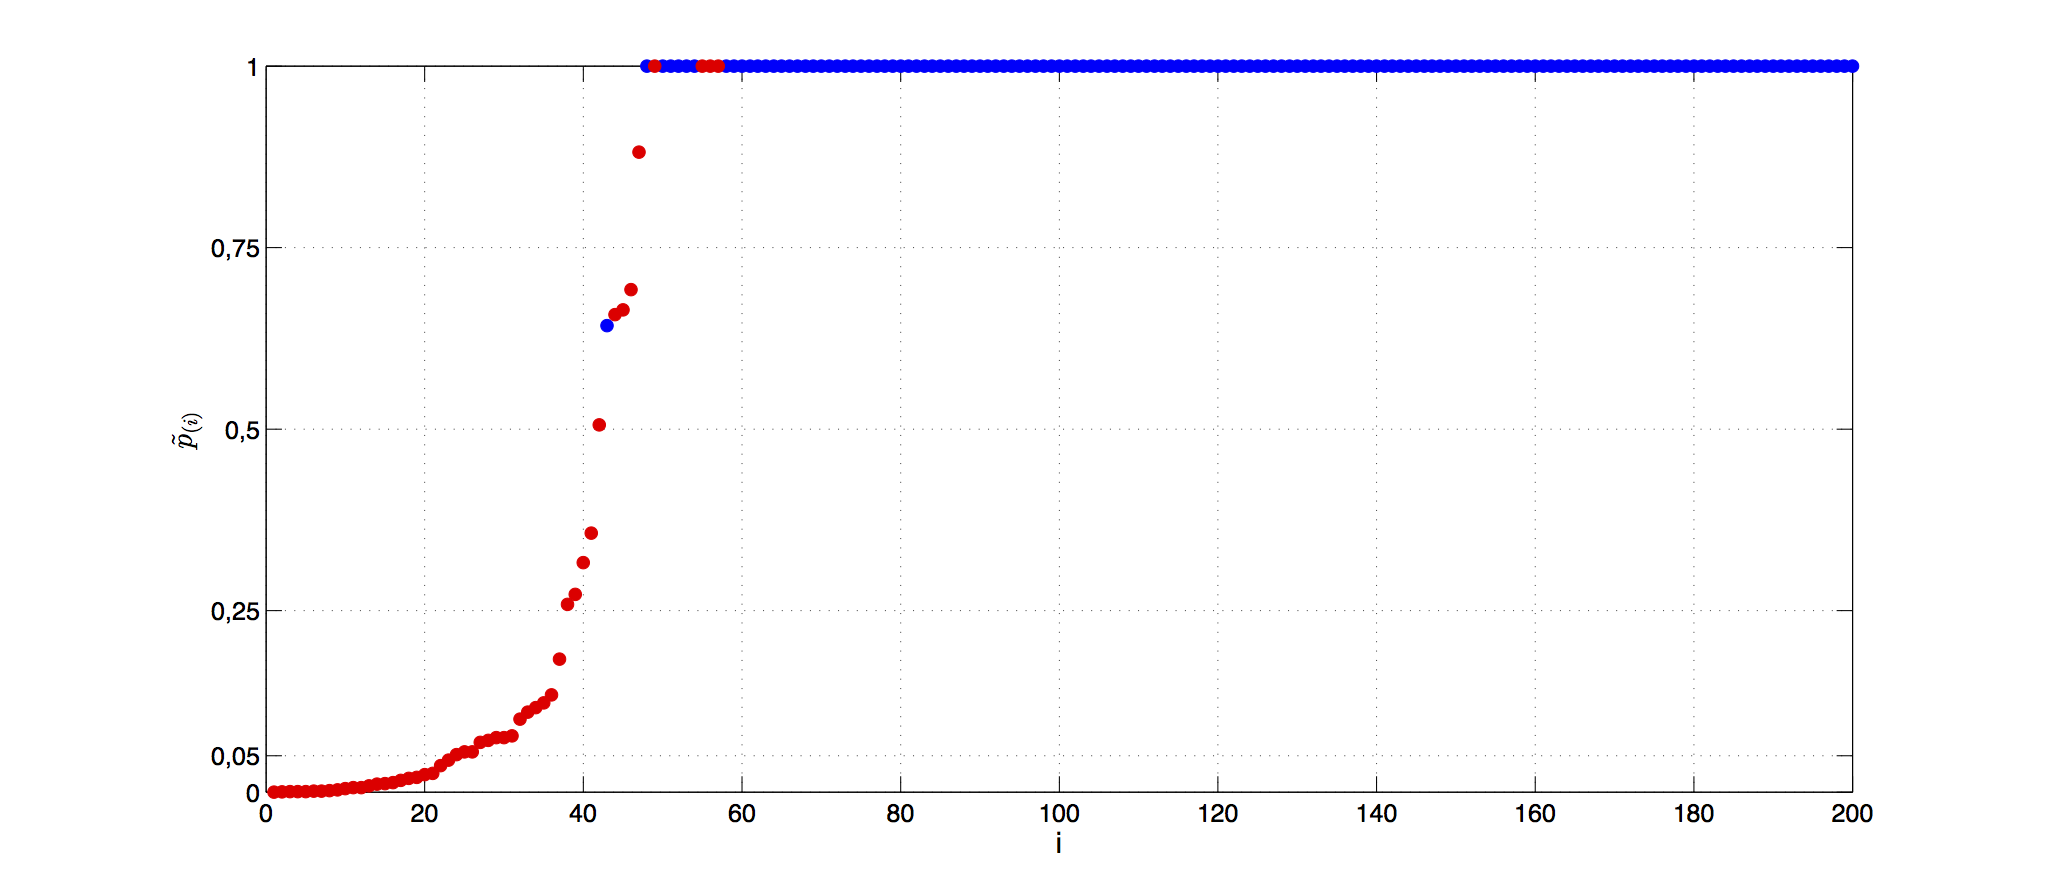
\includegraphics[width=0.8\textwidth]{ps_adj_bonf.png}
    \end{center}

    \begin{center}
        \begin{tabular}{ |r | c | c | c |}
        \hline
                          & Верных $H_i$ & Неверных $H_i$ & Всего \\ \hline
        Принятых $H_i$    & 150          & 27             & 177   \\ \hline
        Отвергнутых $H_i$ & 0            & 23             & 23    \\ \hline
        Всего             & 150          & 50             & 200   \\ \hline
        \end{tabular}
    \end{center}
    }

    \only<3>{
%%%%%%%%%%%%%%%%%%%%%%%%%%%%%%%%%%%%%%%%%%%%%%%%%%%%%%%%%%%%%%%%%%%%%%%
% Метод Холма Этот метод позволил отвергнуть 26 из 50 гипотез и всё ещё не совершить ни одной ошибки первого рода при этом. C одной стороны, разница между методами Холма и Бонферрони. Метод Холма не помог случиться чуду и не отверг все неверные нулевые гипотезы. С другой стороны, этот метод позволил, не делая никаких дополнительных предположений, совершить ещё три открытия. Ещё три гипотезы удалось отвергнуть абсолютно бесплатно. А это уже достаточный повод, чтобы пользоваться этим методом.
%%%%%%%%%%%%%%%%%%%%%%%%%%%%%%%%%%%%%%%%%%%%%%%%%%%%%%%%%%%%%%%%%%%%%%%
    Модифицированные достигаемые уровни значимости, метод Холма:
    \begin{center}
                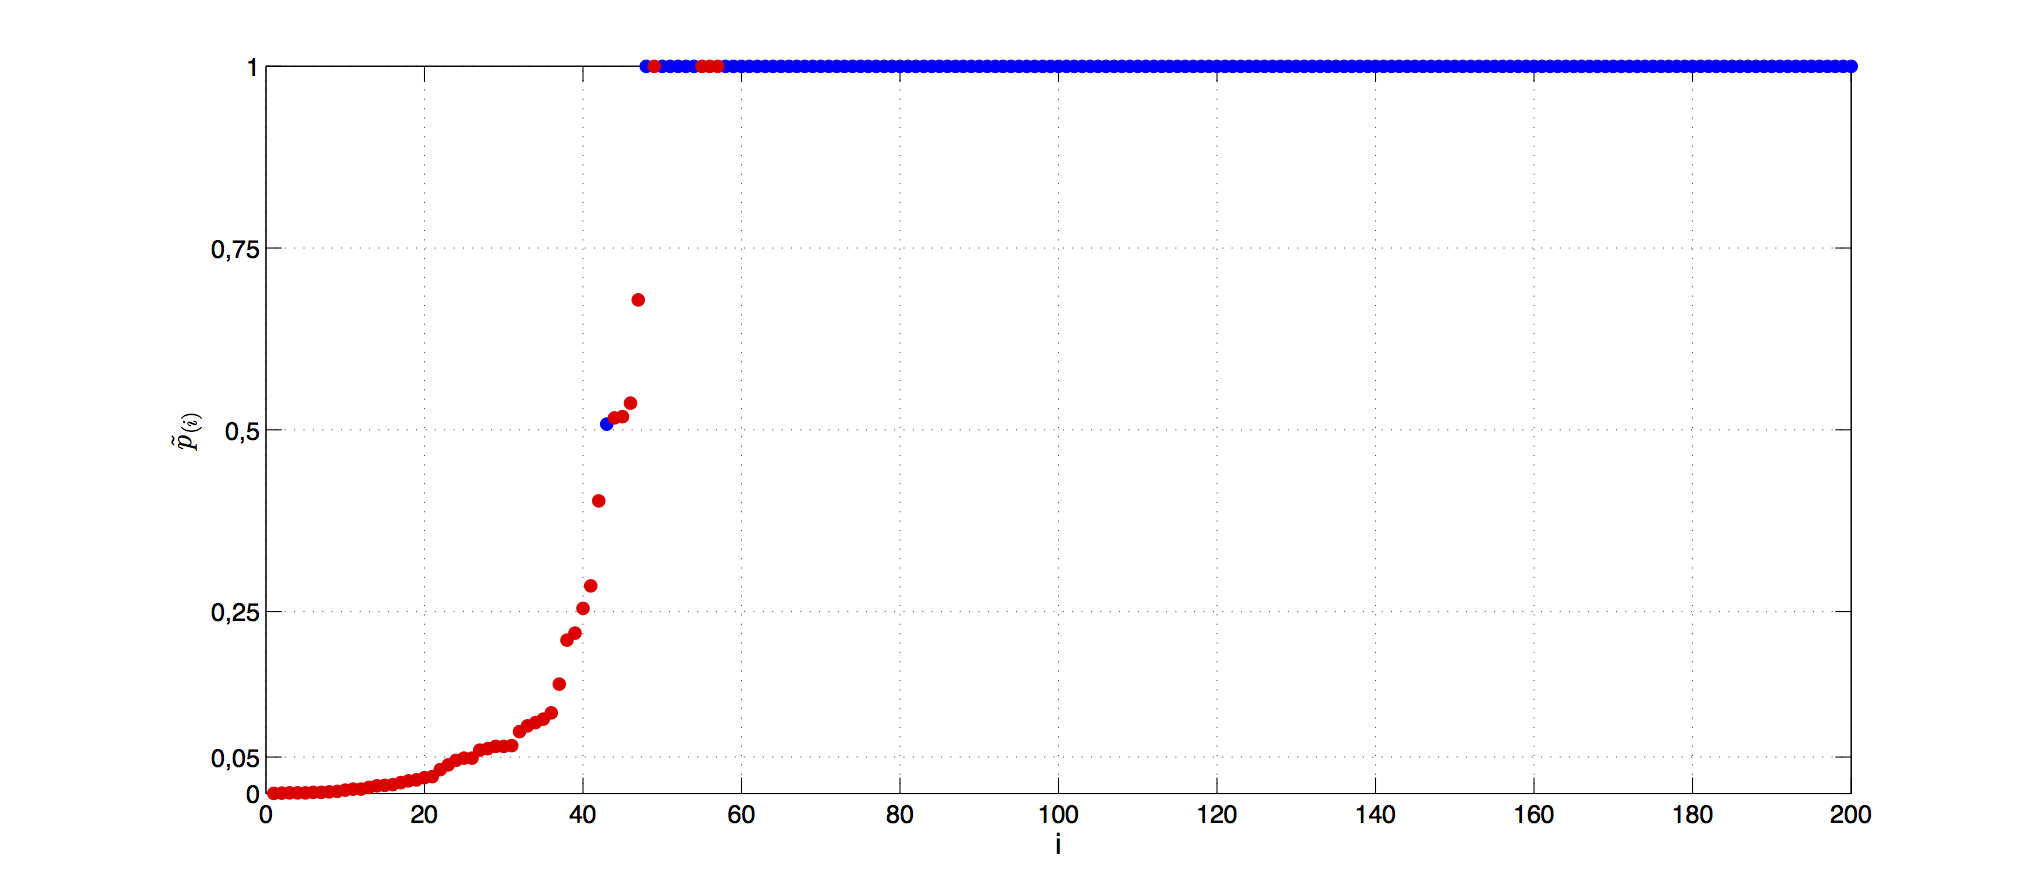
\includegraphics[width=0.8\textwidth]{ps_adj_holm.png}
    \end{center}

    \begin{center}
        \begin{tabular}{ |r | c | c | c |}
        \hline
                          & Верных $H_i$ & Неверных $H_i$ & Всего \\ \hline
        Принятых $H_i$    & 150          & 24             & 174   \\ \hline
        Отвергнутых $H_i$ & 0            & 26             & 26    \\ \hline
        Всего             & 150          & 50             & 200   \\ \hline
        \end{tabular}
    \end{center}
    }
\end{frame}

\begin{frame}{Идеи для дальнейших улучшений}
%%%%%%%%%%%%%%%%%%%%%%%%%%%%%%%%%%%%%%%%%%%%%%%%%%%%%%%%%%%%%%%%%%%%%%%
% Как можно построить более мощную проведуру? Для этого есть несколько путей. Во-первых, вспомним из доказательства теоремы Бонферрони, что FWER на самом деле контролируется на уровне m0/m alpha. То же самое верно и для метода Холма. Если бы мы знали m0, мы могли бы уточнить процедуру. Во-вторых, можно сделать какие-то дополнительные предположения, на основании которых можно построить более мощную процедуру для случаев, когда они выполняются. Наконец, можно попытаться учесть структуру зависимости между статистиками, проверяющими наши гипотезы. Рассмотрим по очереди все три способа. 
%%%%%%%%%%%%%%%%%%%%%%%%%%%%%%%%%%%%%%%%%%%%%%%%%%%%%%%%%%%%%%%%%%%%%%%
    \begin{itemize}
    \item Дополнительно оценить $m_0$.
    \bigskip
    \item Сделать дополнительные предположения:
        \begin{itemize}
        \item о характере зависимости между статистиками;
        \item о совместном распределении статистик.
    \bigskip
        \end{itemize}
    \bigskip
    \item Учесть зависимость между статистиками с помощью перестановочных методов.
    \end{itemize}
\end{frame}

\begin{frame}{Предварительное оценивание $m_0$}
%%%%%%%%%%%%%%%%%%%%%%%%%%%%%%%%%%%%%%%%%%%%%%%%%%%%%%%%%%%%%%%%%%%%%%%
% Метод Шведера-Спьётволла помогает оценить m0. Он основан на интуитивно понятной эвристике: если размер выборки достаточно большой, то большой достигаемый уровень значимости получается у верных гипотез. Возьмём, например, гипотезы с достигаемым уровнем значимости больше 0.5 - с большой вероятностью все соответствующие гипотезы верны. Поскольку при справедливости нулевой гипотезы p-value чаще всего распределены равномерно, то можно предположить, что в нижней половине интервала [0,1] находится примерно столько же верных нулевых гипотез, сколько и в верхней. Итоговая оценка m0 - умноженное на 2 число гипотез с p-value больше 0.5. Порог можно брать равным не 0.5, а произвольному достаточно большому лямбда. 
%%%%%%%%%%%%%%%%%%%%%%%%%%%%%%%%%%%%%%%%%%%%%%%%%%%%%%%%%%%%%%%%%%%%%%%
    Многие методы контролируют $\FWER$ на уровне $\alpha_T=\frac{m_0}{m}\alpha \Rightarrow$ можно оценить $m_0$ и выбрать $\alpha$ так, чтобы $\alpha_T$ было равно желаемой величине.

    \bigskip

    Метод Шведера-Спьётволла: 
    $$\hat{m}_0\left(\lambda\right) = \frac1{1-\lambda}\left(1+\sum_{i=1}^m \left[p_i>\lambda\right]\right), \;\; \lambda \in \left[0,1\right).$$
    %\begin{figure}
    %	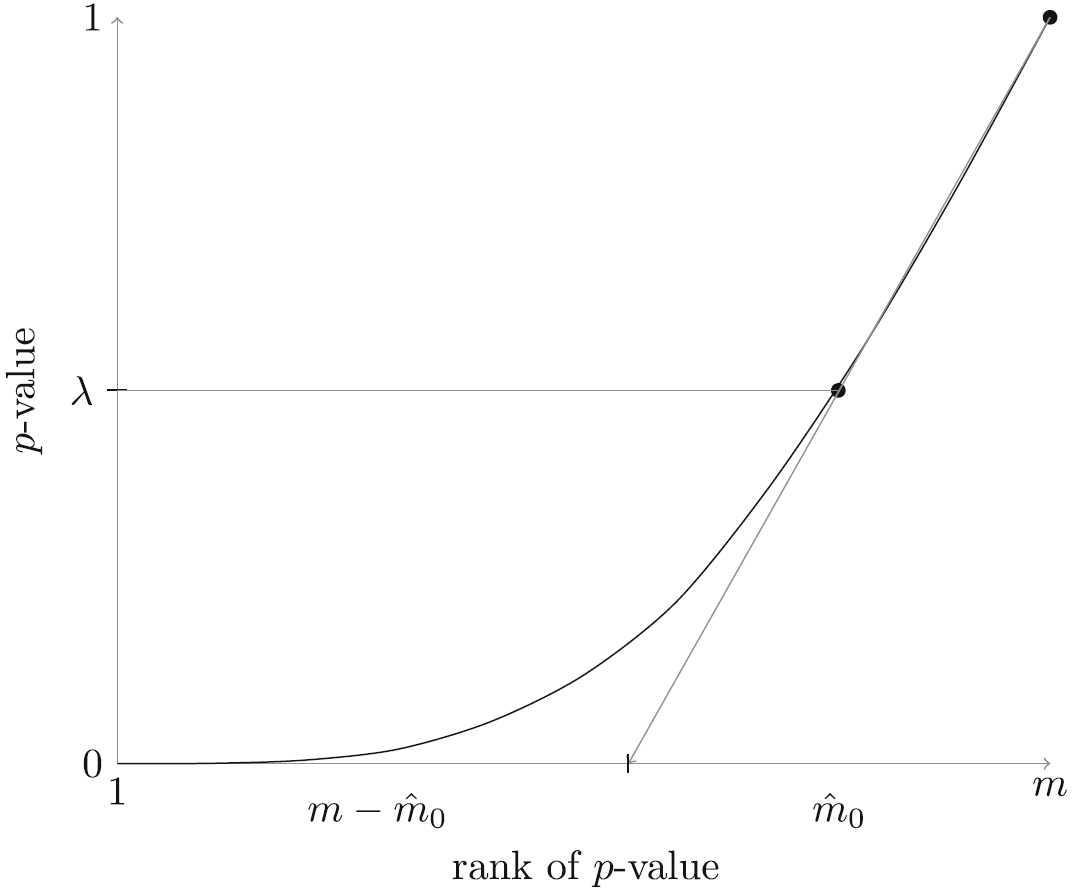
\includegraphics[width=0.45\textwidth]{storey.png}
    %\end{figure}      
    
    Имеет положительное смещение, а также большую дисперсию, особенно при сильно коррелированных $p$, поэтому $\FWER$ не контролируется.
\end{frame}

\begin{frame}{Одношаговый метод Шидака}
	\only<1>{
    \textbf{Метод Шидака}:
    $$\alpha_1 = \alpha_2 = \ldots = \alpha_m = 1-\left(1-\alpha\right)^{\frac1{m}}.$$

    \bigskip
    Идея:
    $$ \FWER\leq \alpha \to P(V>0) \leq \alpha \to 1 - P(V=0) = 1-\left(1-\alpha\right)^{{m}}  \to  \alpha = 1-\left(1-\alpha\right)^{{m}}.$$
    \bigskip

    Метод обеспечивает контроль над $\FWER$ на уровне $\alpha$ при условии, что статистики $T_i$ \textbf{независимы} или выполняется следующее свойство:
    $$P\left(T_1\leq t_1, \dots, T_m \leq t_m\right)\geq \prod_{i=1}^m P\left(T_i\leq t_i\right)\;\; \forall t_1,\dots,t_m$$
    (\textbf{positive lower orthant dependence}).

    \bigskip

    Модифицированные достигаемые уровни значимости:
    $$\tilde{p}_{i} = 1-\left(1-p_i\right)^m.$$
    }    
\end{frame}

\begin{frame}{Нисходящая модификация}
    \only<1>{
    Нисходящий метод Шидака (метод Шидака-Холма)~--- нисходящая процедура со следующими уровнями значимости:
    $$\alpha_1 = 1 - \left(1-\alpha\right)^{\frac1{m}}, \; \ldots, \; \alpha_i = 1 - \left(1-\alpha\right)^{\frac1{m-i+1}}, \; \ldots, \; \alpha_m = \alpha.$$

    \bigskip

    Метод обеспечивает контроль над $\FWER$ на уровне $\alpha$ при условии, что статистики $T_i$ \textbf{независимы}.

    \bigskip

    Модифицированные достигаемые уровни значимости:
    $$\tilde{p}_{(i)} = \max \left(1-\left(1-p_{(i)}\right)^{\left(m-i+1\right)}, \tilde{p}_{(i-1)}\right).$$
    }

    \only<2>{
    На практике при достаточно больших $m$ не слишком отличается от метода Холма:
    \begin{center}
        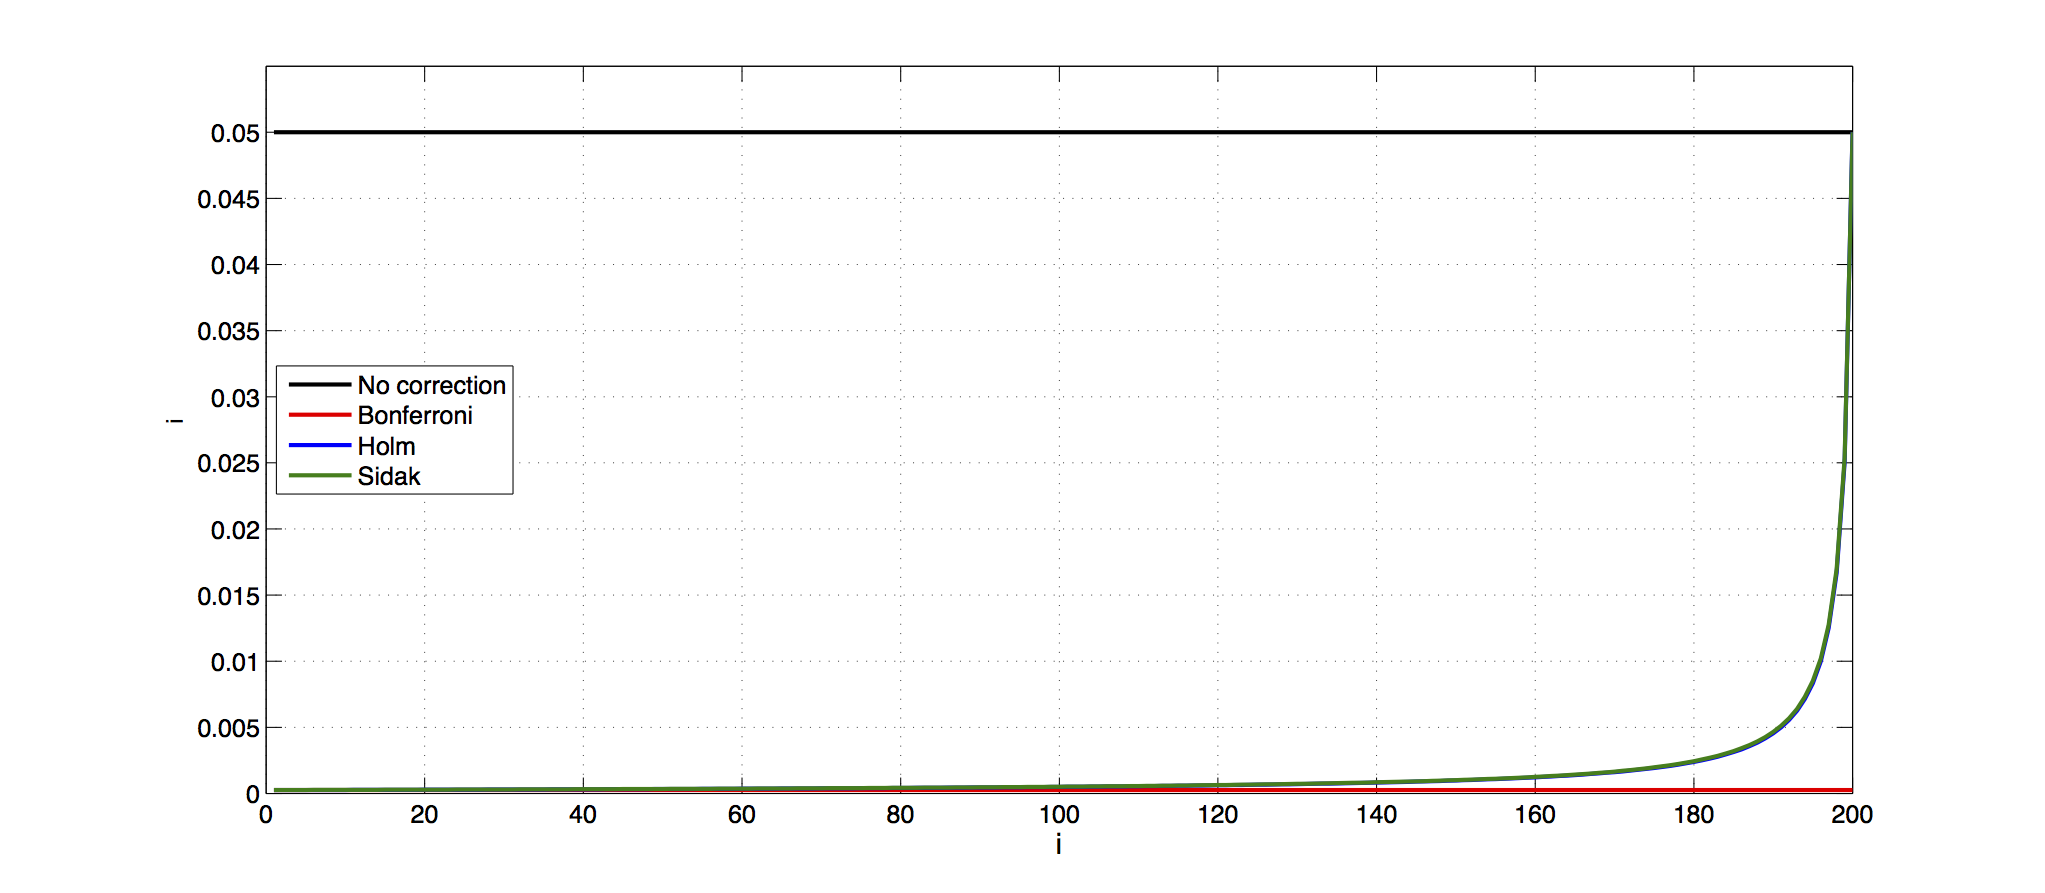
\includegraphics[width=0.85\textwidth]{alphas2.png}
    \end{center}
    }
\end{frame}

\begin{frame}{Модельный эксперимент}
    \only<1>{
    Модифицированные достигаемые уровни значимости, метод Холма:
    \vspace{8.9pt}

    \begin{center}
        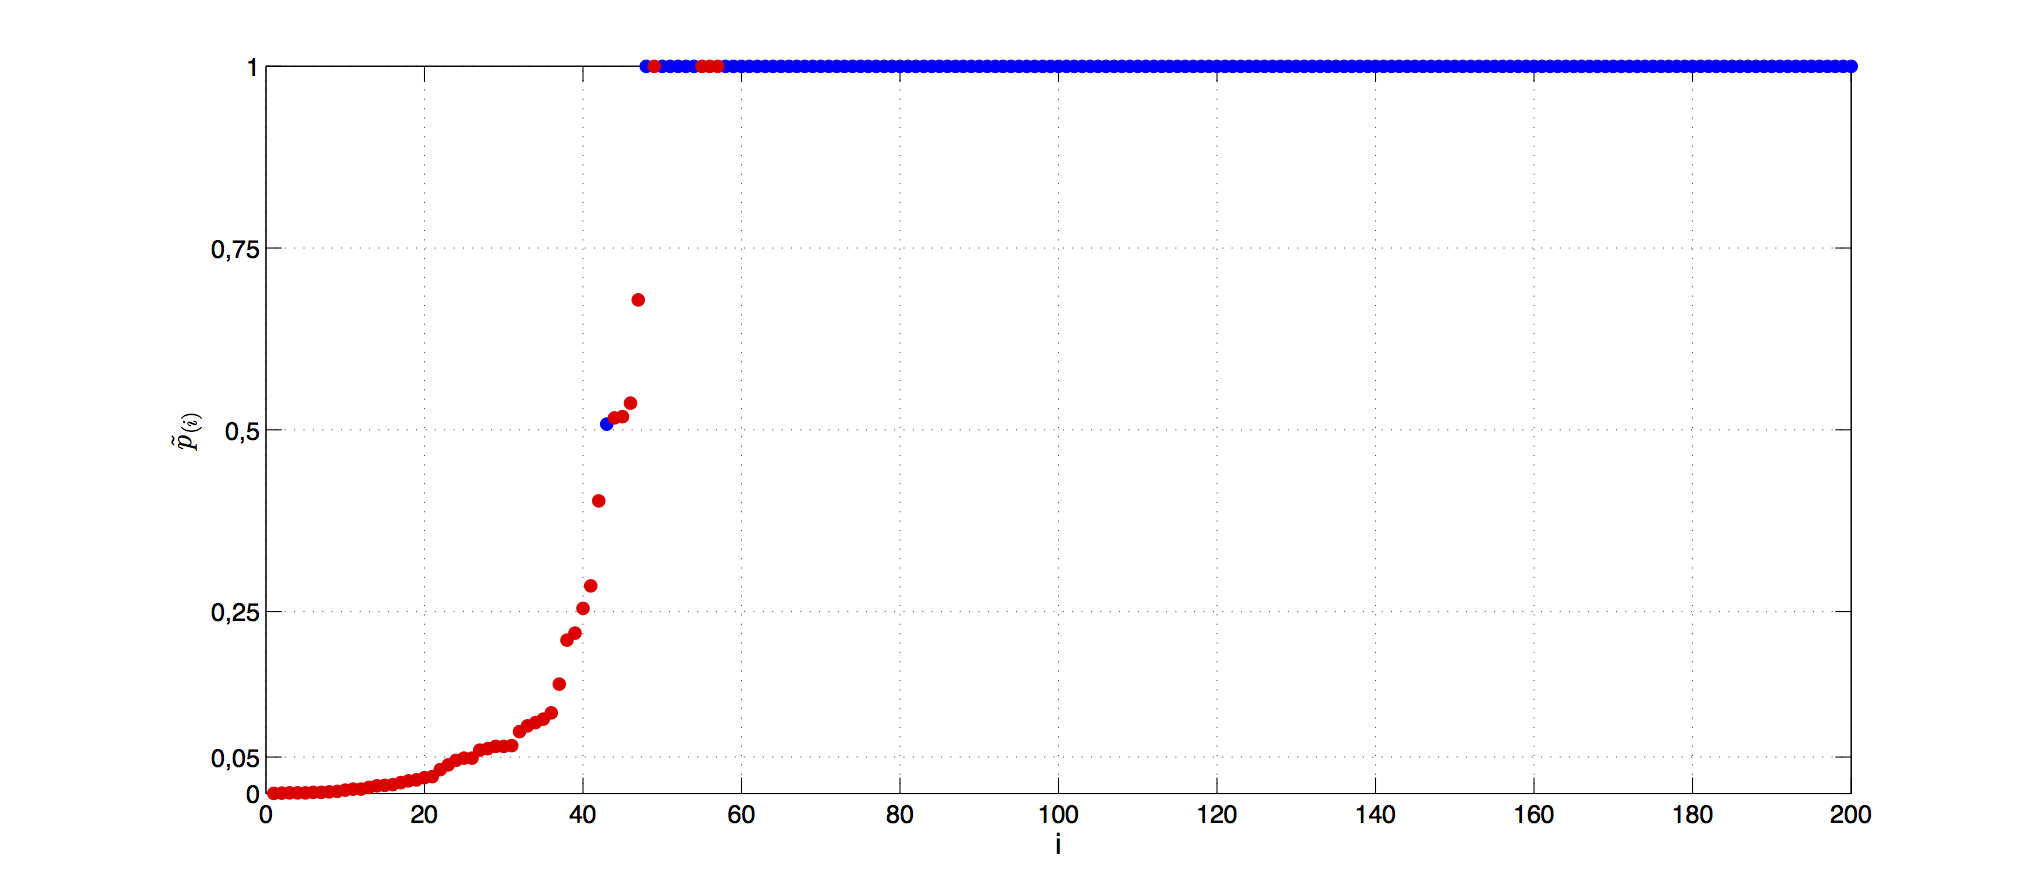
\includegraphics[width=0.8\textwidth]{ps_adj_holm.png}
    \end{center}

    \begin{center}
        \begin{tabular}{ |r | c | c | c |}
        \hline
                          & Верных $H_i$ & Неверных $H_i$ & Всего \\ \hline
        Принятых $H_i$    & 150          & 24             & 174   \\ \hline
        Отвергнутых $H_i$ & 0            & 26             & 26    \\ \hline
        Всего             & 150          & 50             & 200   \\ \hline
        \end{tabular}
    \end{center}
    }

    \only<2>{
%%%%%%%%%%%%%%%%%%%%%%%%%%%%%%%%%%%%%%%%%%%%%%%%%%%%%%%%%%%%%%%%%%%%%%%
% В нашем модельном эксперименте предположение о независимости статистик выполняется - мы это точно знаем, потому что именно так мы сгенерировали данные. Несмотря на это, явный учёт этого свойства в рамках метода Шидака-Холма не позволяет отвергнуть ни одной доролнительной гипотезы к тем, которые отвергаются методом Холма, это предположение не использующим.
%%%%%%%%%%%%%%%%%%%%%%%%%%%%%%%%%%%%%%%%%%%%%%%%%%%%%%%%%%%%%%%%%%%%%%%
    Модифицированные достигаемые уровни значимости, нисходящий метод Шидака:
    \begin{center}
        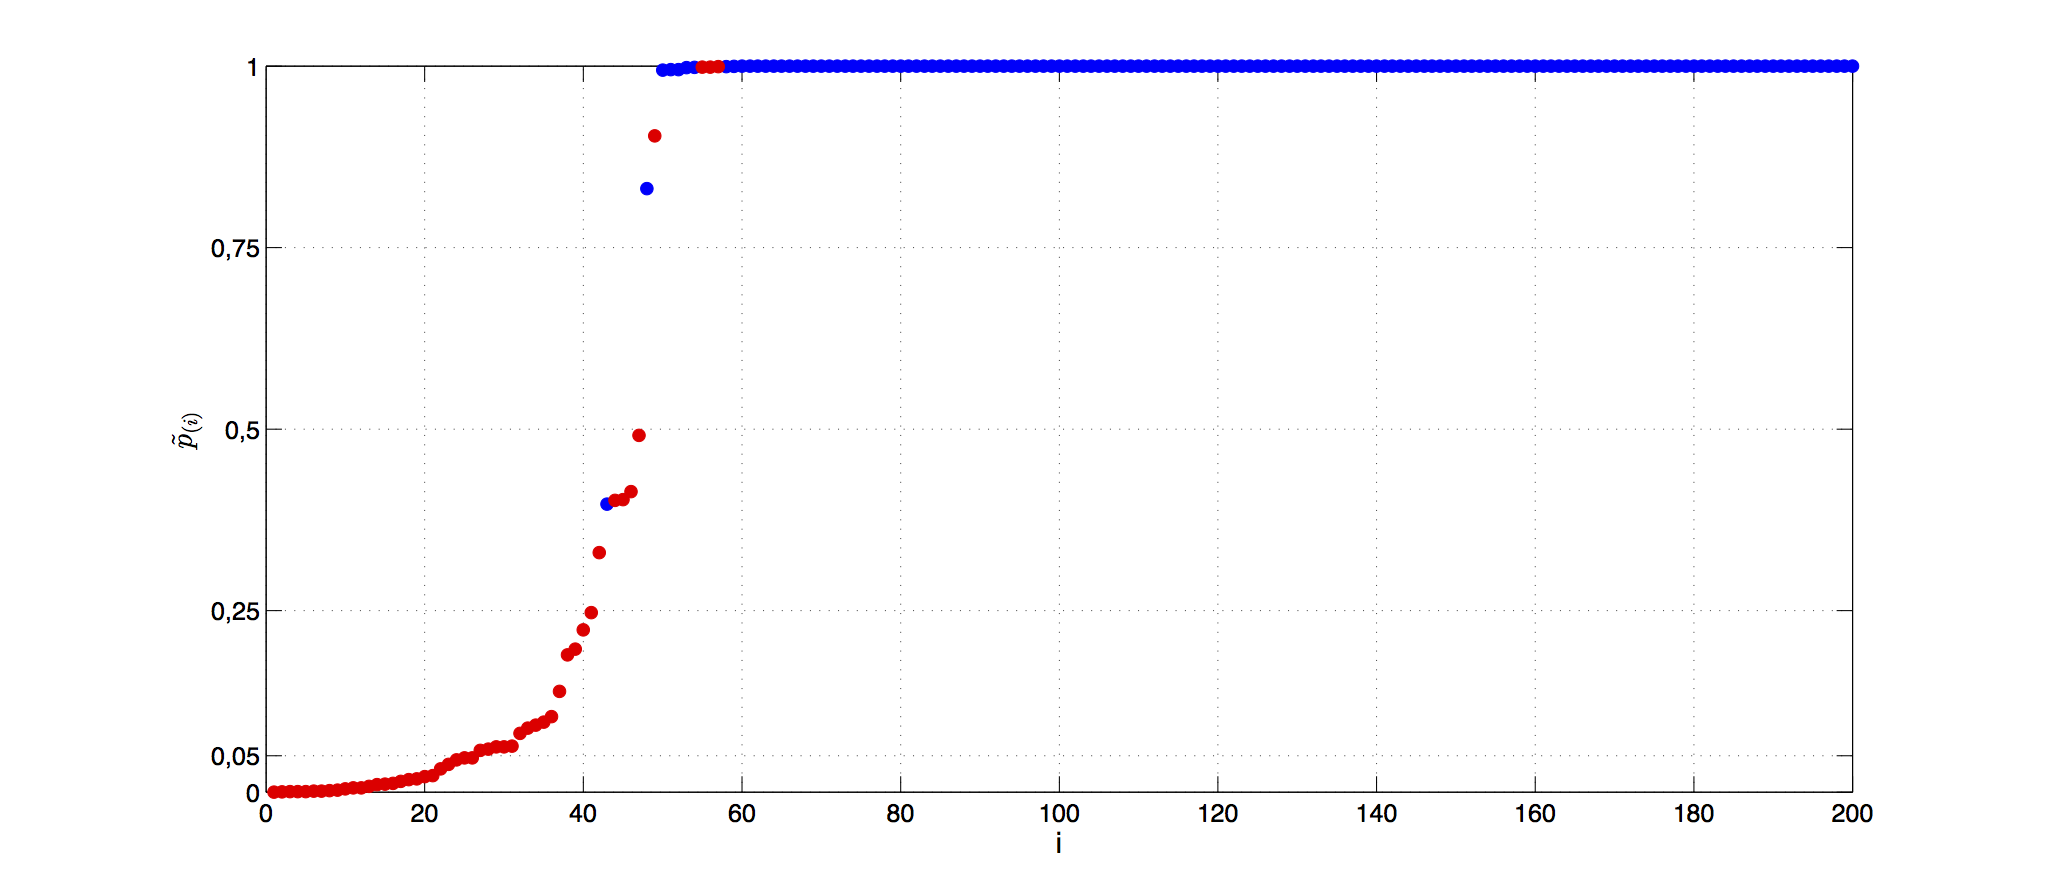
\includegraphics[width=0.8\textwidth]{ps_adj_sidak-holm.png}
    \end{center}

    \begin{center}
        \begin{tabular}{ |r | c | c | c |}
        \hline
                          & Верных $H_i$ & Неверных $H_i$ & Всего \\ \hline
        Принятых $H_i$    & 150          & 24             & 174   \\ \hline
        Отвергнутых $H_i$ & 0            & 26             & 26    \\ \hline
        Всего             & 150          & 50             & 200   \\ \hline
        \end{tabular}
    \end{center}
    }
\end{frame}

\subsection{Учёт зависимостей}
\begin{frame}{Зависимость между статистиками}
    \begin{itemize}
    \item Не учитывая характер зависимости между статистиками, нельзя построить контролирующую $\FWER$ процедуру мощнее, чем метод Холма.
    \item Если статистики независимы, нельзя построить контролирующую $\FWER$ процедуру мощнее, чем метод Шидака-Холма.
    \item Чем сильнее связь между статистиками, тем меньше нужно модицифировать уровни значимости.
    \end{itemize}

    \bigskip

    Для построения мощной процедуры множественной проверки гипотез необходимо учесть структуру зависимости статистик.
\end{frame}



\begin{frame}{Параметрические методы}
%%%%%%%%%%%%%%%%%%%%%%%%%%%%%%%%%%%%%%%%%%%%%%%%%%%%%%%%%%%%%%%%%%%%%%%
% HSD и Даннет ждут нас в лекции про дисперсионный анализ
%%%%%%%%%%%%%%%%%%%%%%%%%%%%%%%%%%%%%%%%%%%%%%%%%%%%%%%%%%%%%%%%%%%%%%%
    Если совместное нулевое распределение статистик $T_1,\ldots,T_m$ известно, константы $\alpha_i$ могут быть так, что контроль над $\FWER$ будет точным ($\FWER=\alpha$).

    \bigskip

    \textbf{Примеры:}
    \begin{itemize}
    \item метод HSD Тьюки для попарных сравнений нормально распределённых выборок друг с другом;
    \item критерий Даннета для сравнения средних $m$ нормально распределённых выборок со средним контрольной выборки.
    \end{itemize}
\end{frame}

\begin{frame}{Перестановочные методы, пример}
\begin{figure}
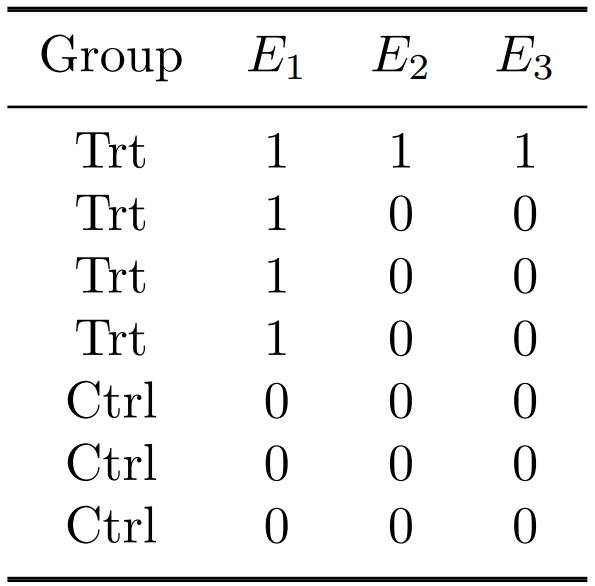
\includegraphics[width=0.3\textwidth]{perm.png}
\caption*{\footnotesize{Источник: Bretz et al.}}
\end{figure}

$p$-value для разных признаков:
\[
    0.02, 0.57, 0.57.
\]



\end{frame}

\begin{frame}{Перестановочные методы}
    Неявно учесть зависимости между статистиками можно при помощи перестановочных методов. Подробнее: Bretz, раздел 5.1.

    \bigskip

     Методы обеспечивают контроль над $\FWER$ на уровне $\alpha$ при условии выполнения свойства \textbf{subset pivotality}:
     $$P\left(\left. \bigcap\limits_{i\in \mathbf{M}^*} \left\{T_i\geq t^* \right\} \right| \bigcap\limits_{i\in \mathbf{M}^*} H_i\right) = P\left(\left. \bigcap\limits_{i\in \mathbf{M}^*} \left\{T_i\geq t^* \right\} \right| \bigcap\limits_{i\in \mathbf{M}} H_i\right) \;\; \forall \mathbf{M}^* \in M$$
     (нулевое распределение любого подмножества статистик $T_i$ не зависит от~того, верны или неверны соответствующие оставшимся статистикам гипотезы).
     
     \bigskip
     
     Примеры задач:
     \begin{itemize}
	     \item проверка гипотез о средних коррелированных нормальных выборок;
	     \item проверка гипотез о линейных комбинациях средних нормальных выборок;
	     \item попарные сравнения средних в нормальных выборках.
     \end{itemize}
\end{frame}


\section{FDR}
\subsection{FDR}
\begin{frame}{Многомерные обобщения ошибки первого рода}
%%%%%%%%%%%%%%%%%%%%%%%%%%%%%%%%%%%%%%%%%%%%%%%%%%%%%%%%%%%%%%%%%%%%%%%
% В описанных ранее поправках при множественном проверке гипотез контролировалась величина групповой вероятности ошибки, то есть ограничивалась вероятность совершить хотя бы одну ошибку первого рода:
% В некоторых ситуациях, например, когда проверяются десятки тысяч или миллионы гипотез, можно допустить какое-то количество ошибок первого рода ради того, чтобы увеличить мощность процедуры и отвергнуть больше неверных гипотез, то есть совершить меньше ошибок второго рода. В таких ситуациях выгоднее использовать другую меру: не familywise error rate, а false discovery rate, ожидаемую долю ложных отклонений:
% Для любой фиксированной процедуры множественной проверки гипотез FDR <= FWER . За счет этого, если контролировать FDR, а не FWER, получается более мощная процедура, поскольку она позволяет отвергать больше гипотез.
%%%%%%%%%%%%%%%%%%%%%%%%%%%%%%%%%%%%%%%%%%%%%%%%%%%%%%%%%%%%%%%%%%%%%%%
    \textbf{Ожидаемая доля ложных отклонений гипотез} (false discovery rate):
    $$\FDR = \mathbb{E}\left(\frac{V}{\max\left(R,1\right)}\right).$$

    \bigskip

    Контроль над ожидаемой долей ложных отклонений на уровне $\alpha$ означает $$\FDR = \mathbb{E}\left(\frac{V}{\max\left(R,1\right)}\right) \leq \alpha ~~\forall P.$$

    \bigskip

    Для любой процедуры множественной проверки гипотез $\FDR\leq \FWER.$
\end{frame}

\subsection{Восходящие методы}
\begin{frame}{Восходящие методы множественной проверки гипотез}
\only<1>{
%%%%%%%%%%%%%%%%%%%%%%%%%%%%%%%%%%%%%%%%%%%%%%%%%%%%%%%%%%%%%%%%%%%%%%%
% Восходящие методы работают с тем же самым вариационным рядом достигаемых уровней значимости, что и нисходящие:
% Отличие заключается в том, что процедура начинается с другого конца этого ряда. На первом шаге самый большой p-value pm сравнивается с соответствующей ему константой альфаm. Если p(m) ? альфаm, то все нулевые гипотезы H(1), H(2), . . . , H(m) отвергаются, и процедура останавливается. Иначе гипотеза H(m) принимает- ся, и процедура продолжается. На следующем шаге сравниваются p(m?1) и альфаm?1. Если p(m?1) ? альфаm?1, то все нулевые гипотезы H(1), H(2), . . . , H(m?1) отвергаются, и процедура останавливается. Иначе принимается гипотеза H(m?1), процедура продолжается. И так далее.
%%%%%%%%%%%%%%%%%%%%%%%%%%%%%%%%%%%%%%%%%%%%%%%%%%%%%%%%%%%%%%%%%%%%%%%
    Составим вариационный ряд достигаемых уровней значимости: $$p_{(1)}\leq p_{(2)} \leq \ldots \leq p_{(m)},$$
    $H_{(1)}, H_{(2)}, \ldots, H_{(m)}$~--- соответствующие гипотезы.

    \bigskip

    \begin{enumerate}
    \item Если $p_{(m)}\leq\alpha_m,$ отвергнуть все нулевые гипотезы $H_{(1)}, H_{(2)}, \ldots, H_{(m)}$ и~остановиться; иначе принять $H_{(m)}$ и~продолжить.
    \item Если $p_{(m-1)}\leq\alpha_{m-1},$ отвергнуть все нулевые гипотезы $H_{(1)}, H_{(2)}, \ldots, H_{(m-1)}$ и~остановиться; иначе принять $H_{(m-1)}$ и~продолжить.
    \item \ldots
    \end{enumerate}

    \bigskip

    Каждый достигаемый уровень значимости $p_{(i)}$ сравнивается со своим уровнем значимости $\alpha_i$.
    }
    
    \only<2>{
%%%%%%%%%%%%%%%%%%%%%%%%%%%%%%%%%%%%%%%%%%%%%%%%%%%%%%%%%%%%%%%%%%%%%%%
% Если для одних и тех же альфаi построить восходящую и нисходящую процедуру, то восходящая процедура всегда будет отвергать не меньше гипотез, чем нисходящая. На рисунке показано, какие гипотезы отвергаются восходящими и нисходящими методами. При использовании восходящей процедуры движение происходит от самого большого p-value к самому маленькому. В таком случае принимаются гипотезы H9,H8,H7. Если ис- пользуется нисходящая процедура, то наоборот, всё начинается с самого маленького p-value, и первые две гипотезы отвергаются, а оставшиеся семь — принимаются. Таким образом, в этом примере восходящая про- цедура отвергла в три раза больше гипотез, чем нисходящая. Это может просходить из-за того, что линия, соединяющая отсортированные достигаемые уровни значимости, может несколько раз пересекать прямую, задающую критические значения альфа.
%%%%%%%%%%%%%%%%%%%%%%%%%%%%%%%%%%%%%%%%%%%%%%%%%%%%%%%%%%%%%%%%%%%%%%%
    Восходящая процедура всегда отвергает не меньше гипотез, чем нисходящая с теми же уровнями значимости:
    \begin{figure}
    	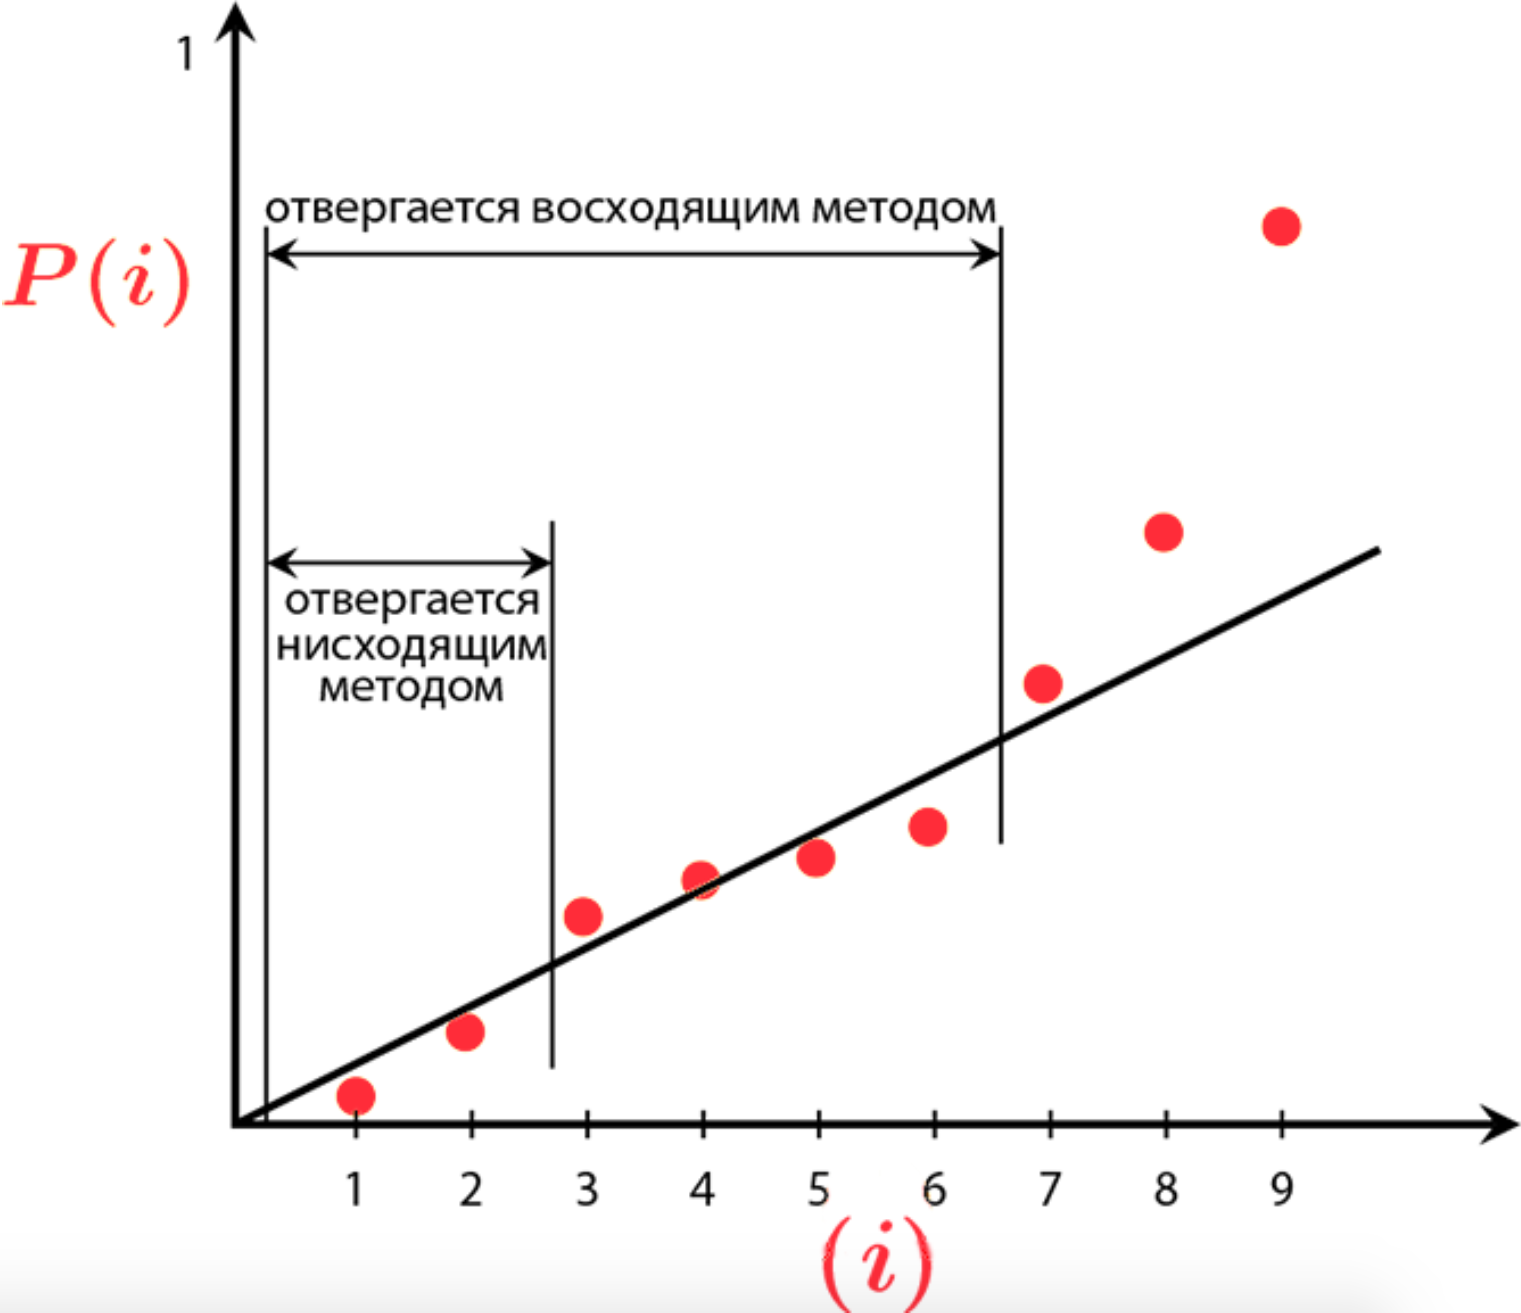
\includegraphics[width=0.5\textwidth]{stepupdown.png}
    \end{figure}    
    }
\end{frame}

\begin{frame}{Метод Бенджамини-Хохберга}
    \only<1>{
%%%%%%%%%%%%%%%%%%%%%%%%%%%%%%%%%%%%%%%%%%%%%%%%%%%%%%%%%%%%%%%%%%%%%%%
% Для контроля над FDR чаще всего используется метод Бенджамини-Хохберга. Это восходящая процедура с уровнями значимости ...
% Модифицированные достигаемые уровни значимости для метода Бенджамини-Хохберга выглядят следующим образом:
% Процедура восходящая, и каждый следующий p-value в ней не должен стать больше, чем предыдущий, поэтому берётся минимум .
% Метод Бенджамини-Хохберга обеспечивает контроль над FDR на уровне альфа только при условии независимости статистик, которые проверяют гипотезы. Это требование достаточно сильное. Иногда его можно ослабить до так называемого свойства PRDS, и в некоторых задачах выполняется ослабленное требование. Тем не менее, важно подчеркнуть, что процедура Бенджамини-Хохберга не является универсальной и она не применима безусловно, в отличие метода Холма.
%%%%%%%%%%%%%%%%%%%%%%%%%%%%%%%%%%%%%%%%%%%%%%%%%%%%%%%%%%%%%%%%%%%%%%%
    Метод Бенджамини-Хохберга~--- восходящая процедура со следующими уровнями значимости:
    $$\alpha_1 = \frac{\alpha}{m}, \; \ldots, \; \alpha_i = \frac{\alpha i}{m}, \; \ldots, \; \alpha_m = \alpha.$$

    \bigskip

    Метод обеспечивает контроль над $\FDR$ на уровне $\alpha$ при условии, что статистики $T_i$ \textbf{независимы} или выполняется следующее свойство:
    $$P\left(X\in D\left|T_i=x\right.\right)\text{ неубывает по } x \;\; \forall i\in M_0,$$
    где $D$~--- произвольное возрастающее множество, то есть, такое, что из~$x\in D$ и $y\geq x$ следует $y\in D$.

    (\textbf{PRDS on $T_i, i\in M_0$} (positive regression dependency on each one from a~subset)).

    \bigskip

    Модифицированные достигаемые уровни значимости:
    $$\tilde{p}_{(i)} = \min \left(1, \frac{mp_{(i)}}{i}, \tilde{p}_{(i+1)}\right).$$
    }
	
	\only<2>{
	PRDS выполняется, например, для многомерного нормального распределения с нулевыми средними и неотрицательными корреляциями элементов из $M_0$, а также для некоторых его производных.
	
	\bigskip
	
	Примеры задач:
	\begin{itemize}
		\item анализ непересекающихся подгрупп при сравнении двух выборок критерием Стьюдента с общей оценкой дисперсии;
		\item сравнение одной нормальной выборки с многими при использовании общей оценки дисперсии;		
	\end{itemize}
	}
	
    \only<3>{
%%%%%%%%%%%%%%%%%%%%%%%%%%%%%%%%%%%%%%%%%%%%%%%%%%%%%%%%%%%%%%%%%%%%%%%
% Крайние уровни значимости точно также же, как и в методе Холма, а вот между ними — абсолютно другие. В методе Бенджамини-Хохберга уровни значимости между альфа1 и альфаm меняются линейно, в то время как в методе Холма — по гиперболе.
%%%%%%%%%%%%%%%%%%%%%%%%%%%%%%%%%%%%%%%%%%%%%%%%%%%%%%%%%%%%%%%%%%%%%%%
    \begin{center}
        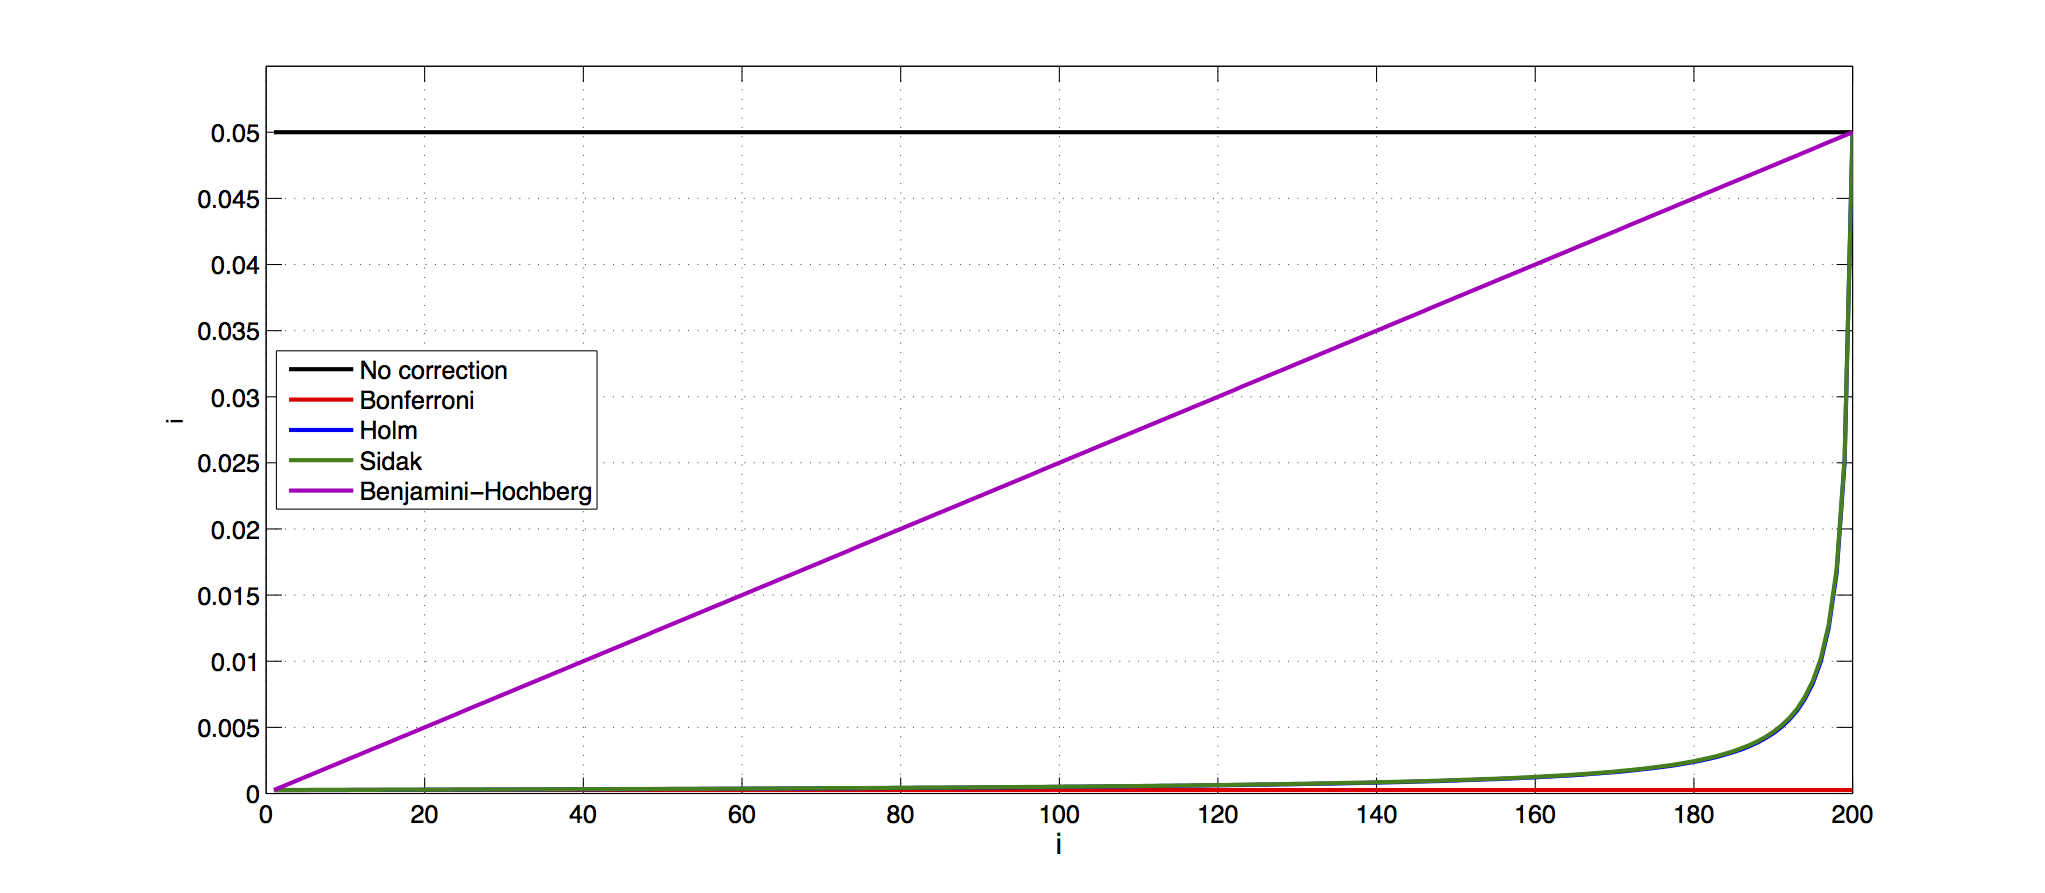
\includegraphics[width=\textwidth]{alphas3.png}
    \end{center}
    }
\end{frame}

\begin{frame}{Модельный эксперимент}
    \only<1>{
    Модифицированные достигаемые уровни значимости, метод Холма:
    \vspace{8.9pt}

    \begin{center}
        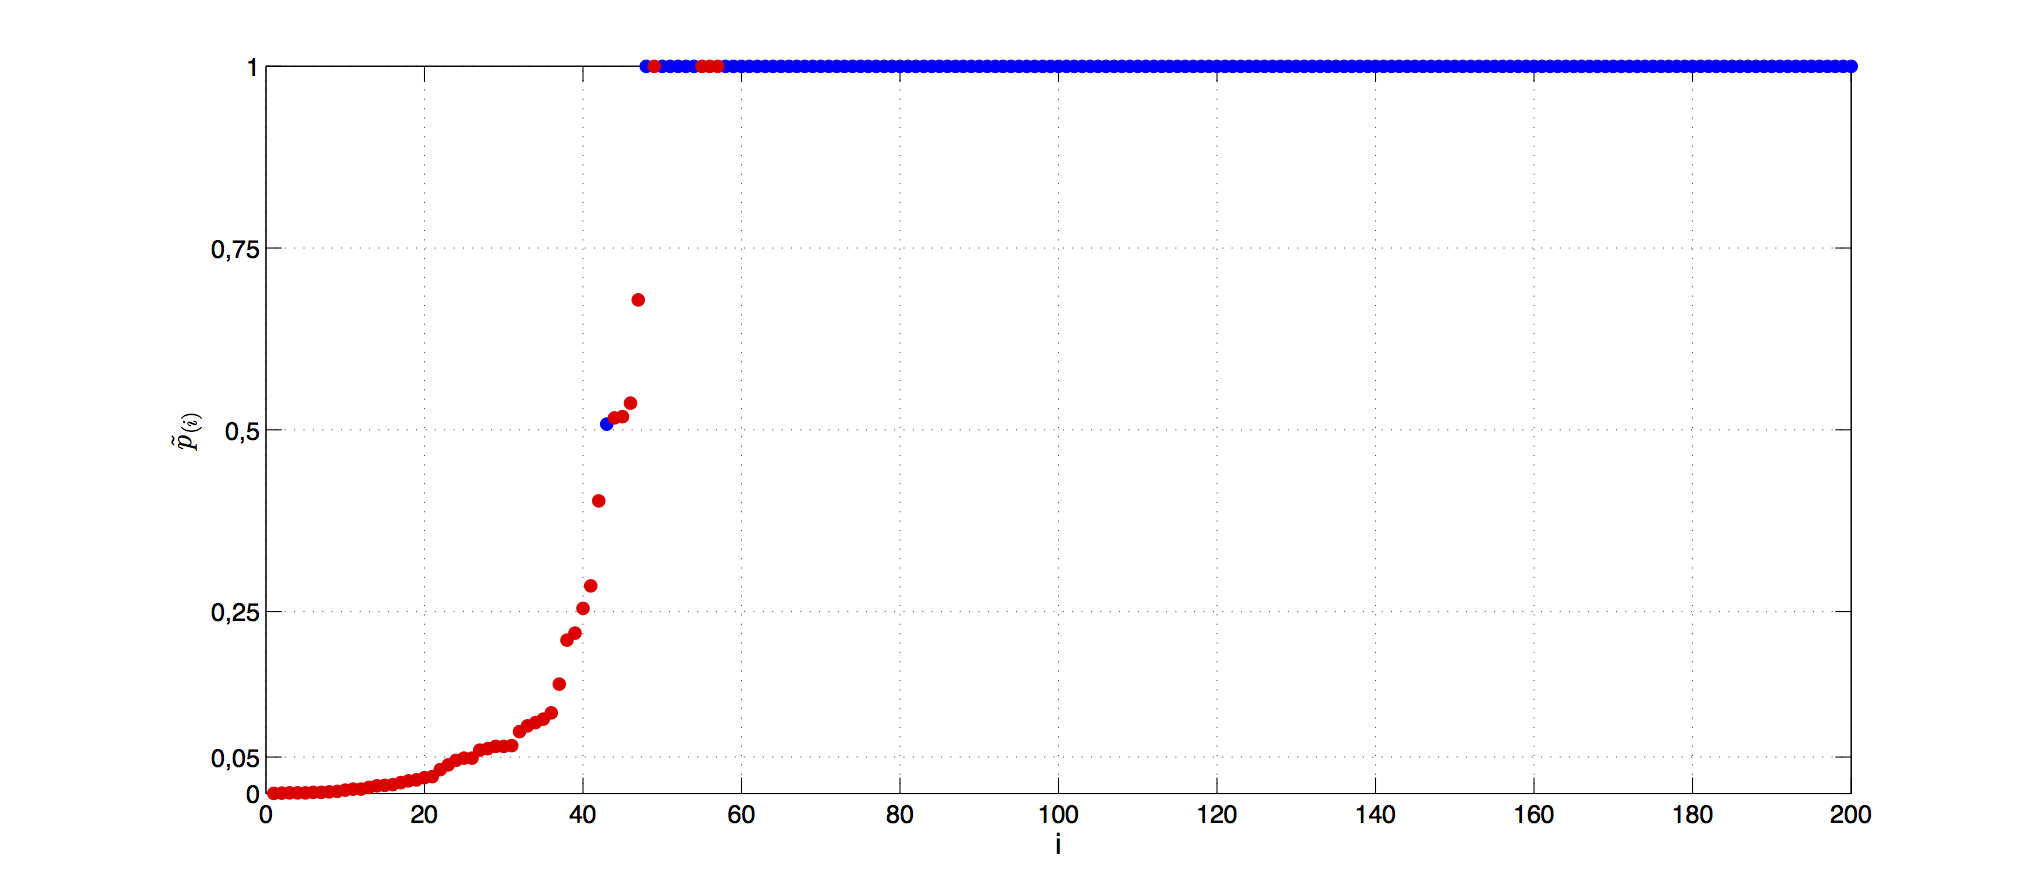
\includegraphics[width=0.8\textwidth]{ps_adj_holm.png}
    \end{center}

    \begin{center}
        \begin{tabular}{ |r | c | c | c |}
        \hline
                          & Верных $H_i$ & Неверных $H_i$ & Всего \\ \hline
        Принятых $H_i$    & 150          & 24             & 174   \\ \hline
        Отвергнутых $H_i$ & 0            & 26             & 26    \\ \hline
        Всего             & 150          & 50             & 200   \\ \hline
        \end{tabular}
    \end{center}
    }

    \only<2>{
    Модифицированные достигаемые уровни значимости, метод Бенджамини-Хохберга:
    \begin{center}
		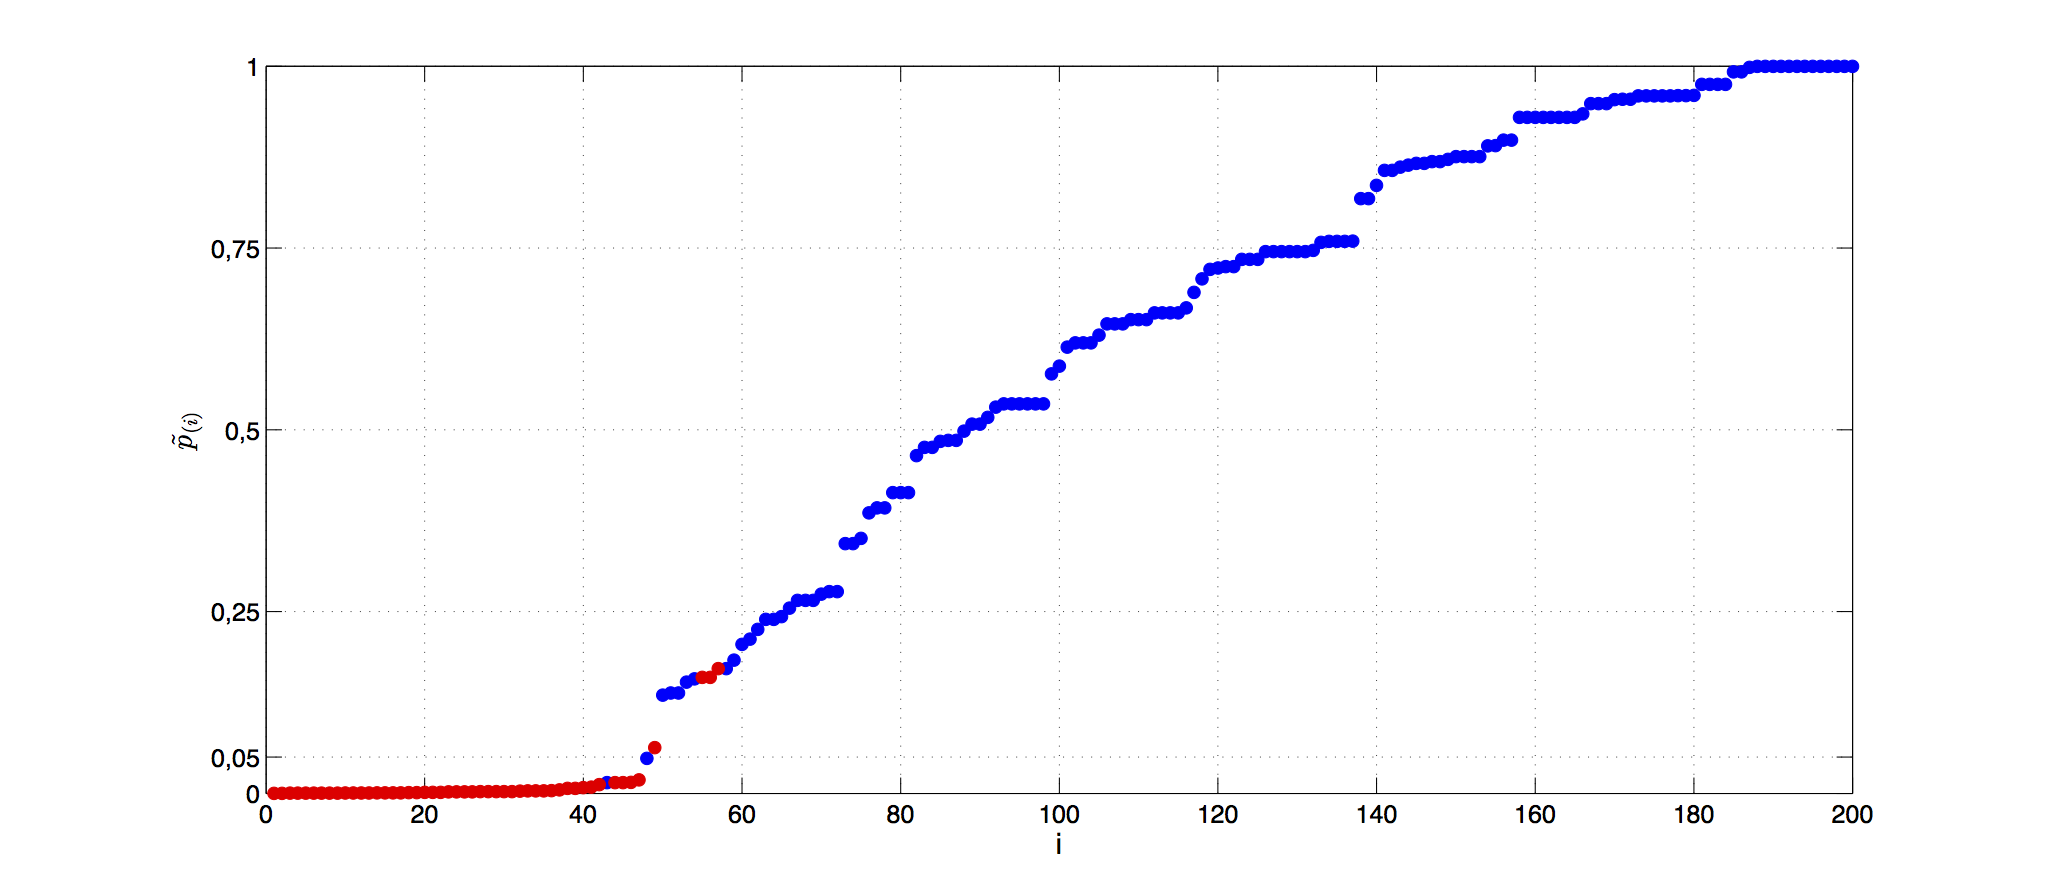
\includegraphics[width=0.8\textwidth]{ps_adj_bh.png}
    \end{center}

    \begin{center}
        \begin{tabular}{ |r | c | c | c |}
        \hline
                          & Верных $H_i$ & Неверных $H_i$ & Всего \\ \hline
        Принятых $H_i$    & 148          & 4              & 152   \\ \hline
        Отвергнутых $H_i$ & 2            & 46             & 48    \\ \hline
        Всего             & 150          & 50             & 200   \\ \hline
        \end{tabular}
    \end{center}
    }
\end{frame}

\begin{frame}{Метод Бенджамини-Иекутиели}
    \only<1>{
    Метод Бенджамини-Иекутиели~--- восходящая процедура со следующими уровнями значимости:
    $$\alpha_1 = \frac{\alpha}{m \sum\limits_{j=1}^m \frac1{j}}, \; \ldots, \; \alpha_i = \frac{\alpha i}{m \sum\limits_{j=1}^m \frac1{j} }, \; \ldots, \; \alpha_m = \frac{\alpha}{\sum\limits_{j=1}^m \frac1{j}}.$$

    \bigskip

    Метод обеспечивает контроль над $\FDR$ на уровне $\frac{m_0}{m}\alpha\leq\alpha$ при любых $p_i$ и $T_i$. 
    При отсутствии информации о зависимости между статистиками метод неулучшаем.

    \bigskip

    Модифицированные достигаемые уровни значимости:
    $$\tilde{p}_{(i)} = \min \left(1, \frac{mp_{(i)} \sum\limits_{j=1}^m \frac1{j} }{i}, \tilde{p}_{(i+1)}\right).$$
    \bigskip
    Если доля неверных гипотез мала, метод Бенджамини-Иекутиели отвергает меньше гипотез, чем метод Холма.
    }

    \only<2>{
    \begin{center}
        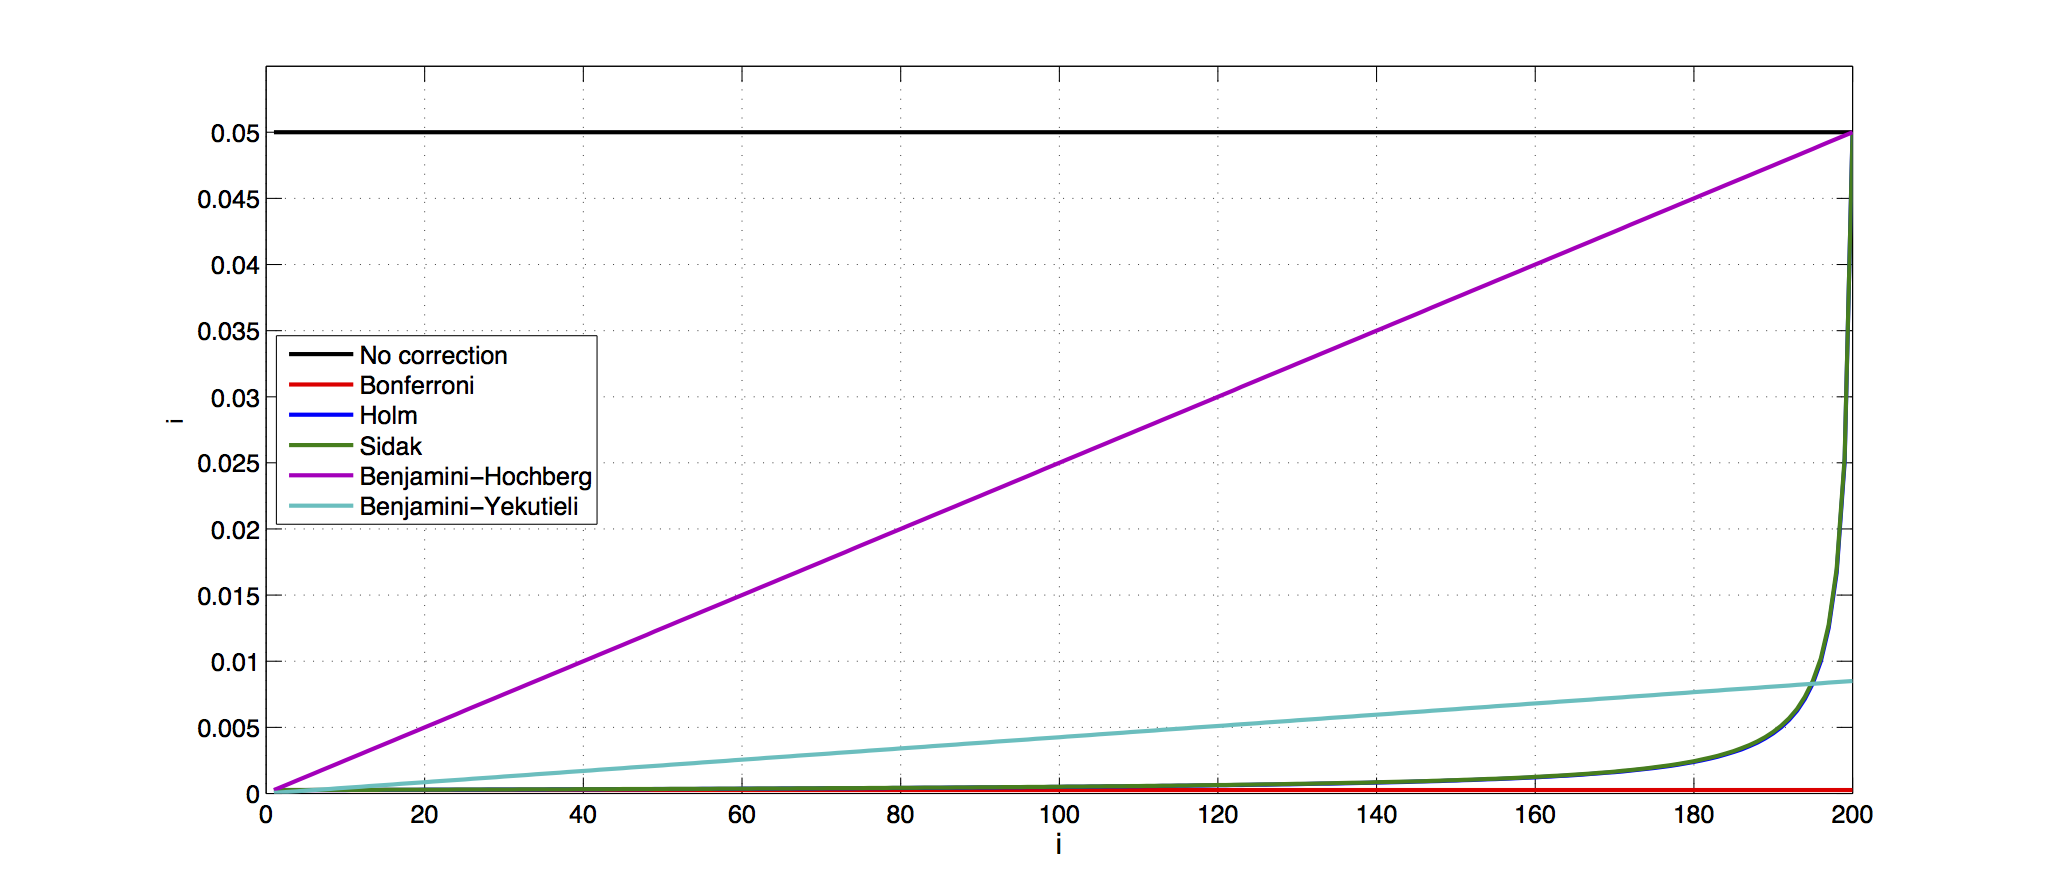
\includegraphics[width=0.8\textwidth]{alphas4.png}
    \end{center}
    }
\end{frame}

\begin{frame}{Модельный эксперимент}
    \only<1>{
    Модифицированные достигаемые уровни значимости, метод Холма:
    \vspace{8.9pt}

    \begin{center}
        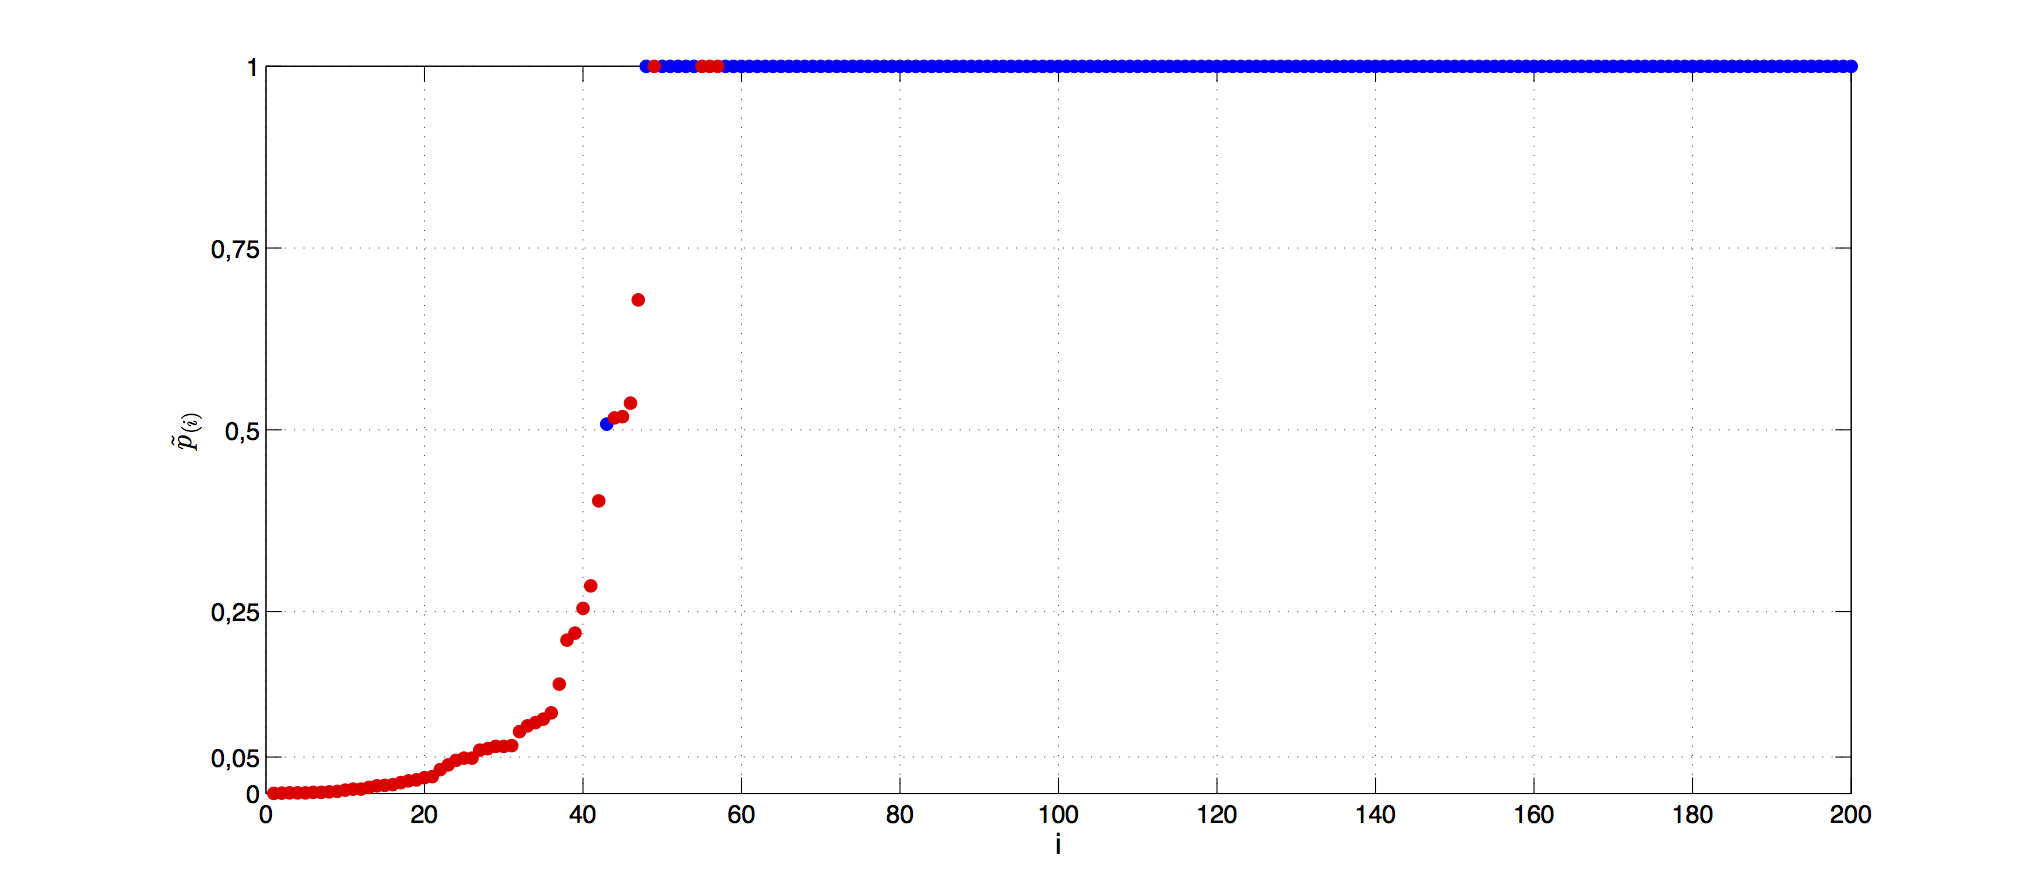
\includegraphics[width=0.8\textwidth]{ps_adj_holm.png}
    \end{center}

    \begin{center}
        \begin{tabular}{ |r | c | c | c |}
        \hline
                          & Верных $H_i$ & Неверных $H_i$ & Всего \\ \hline
        Принятых $H_i$    & 150          & 24             & 174   \\ \hline
        Отвергнутых $H_i$ & 0            & 26             & 26    \\ \hline
        Всего             & 150          & 50             & 200   \\ \hline
        \end{tabular}
    \end{center}
    }

    \only<2>{
    Модифицированные достигаемые уровни значимости, нисходящий метод Бенджамини-Хохберга:
    \begin{center}
        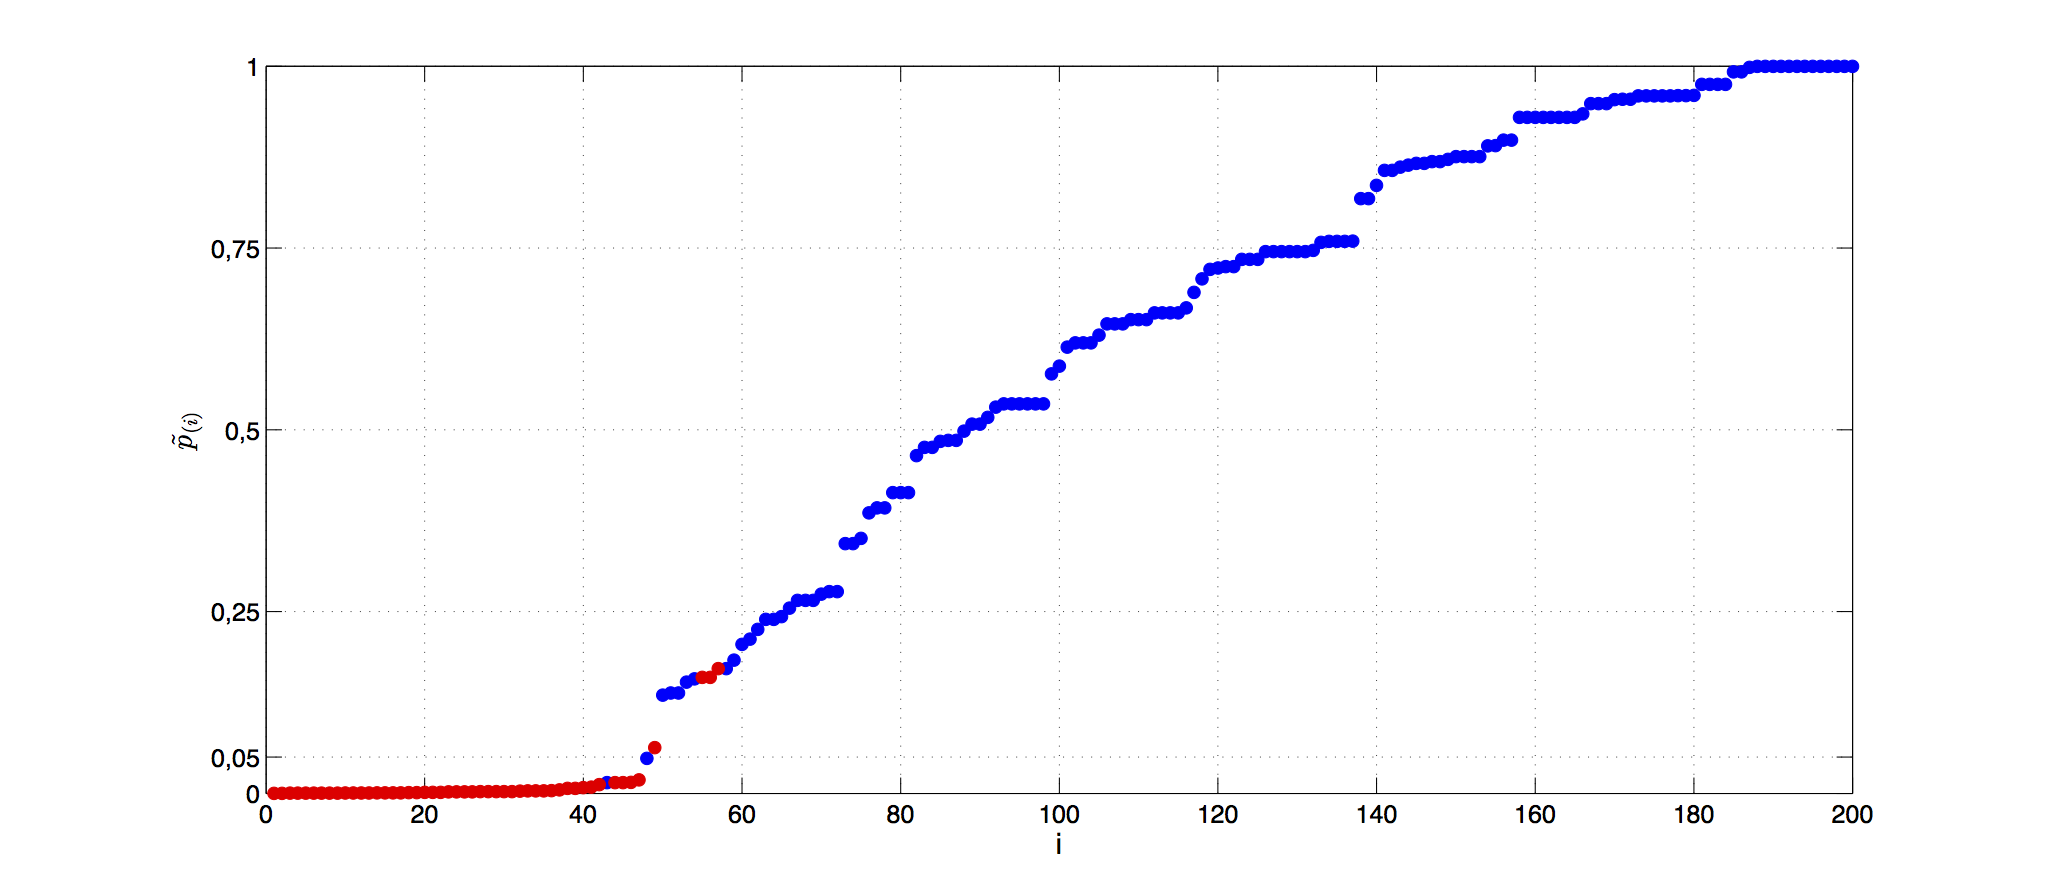
\includegraphics[width=0.8\textwidth]{ps_adj_bh.png}
    \end{center}

    \begin{center}
        \begin{tabular}{ |r | c | c | c |}
        \hline
                          & Верных $H_i$ & Неверных $H_i$ & Всего \\ \hline
        Принятых $H_i$    & 148          & 4              & 152   \\ \hline
        Отвергнутых $H_i$ & 2            & 46             & 48    \\ \hline
        Всего             & 150          & 50             & 200   \\ \hline
        \end{tabular}
    \end{center}
    }

    \only<3>{
    Модифицированные достигаемые уровни значимости, нисходящий метод Бенджамини-Иекутиели:
    \begin{center}
        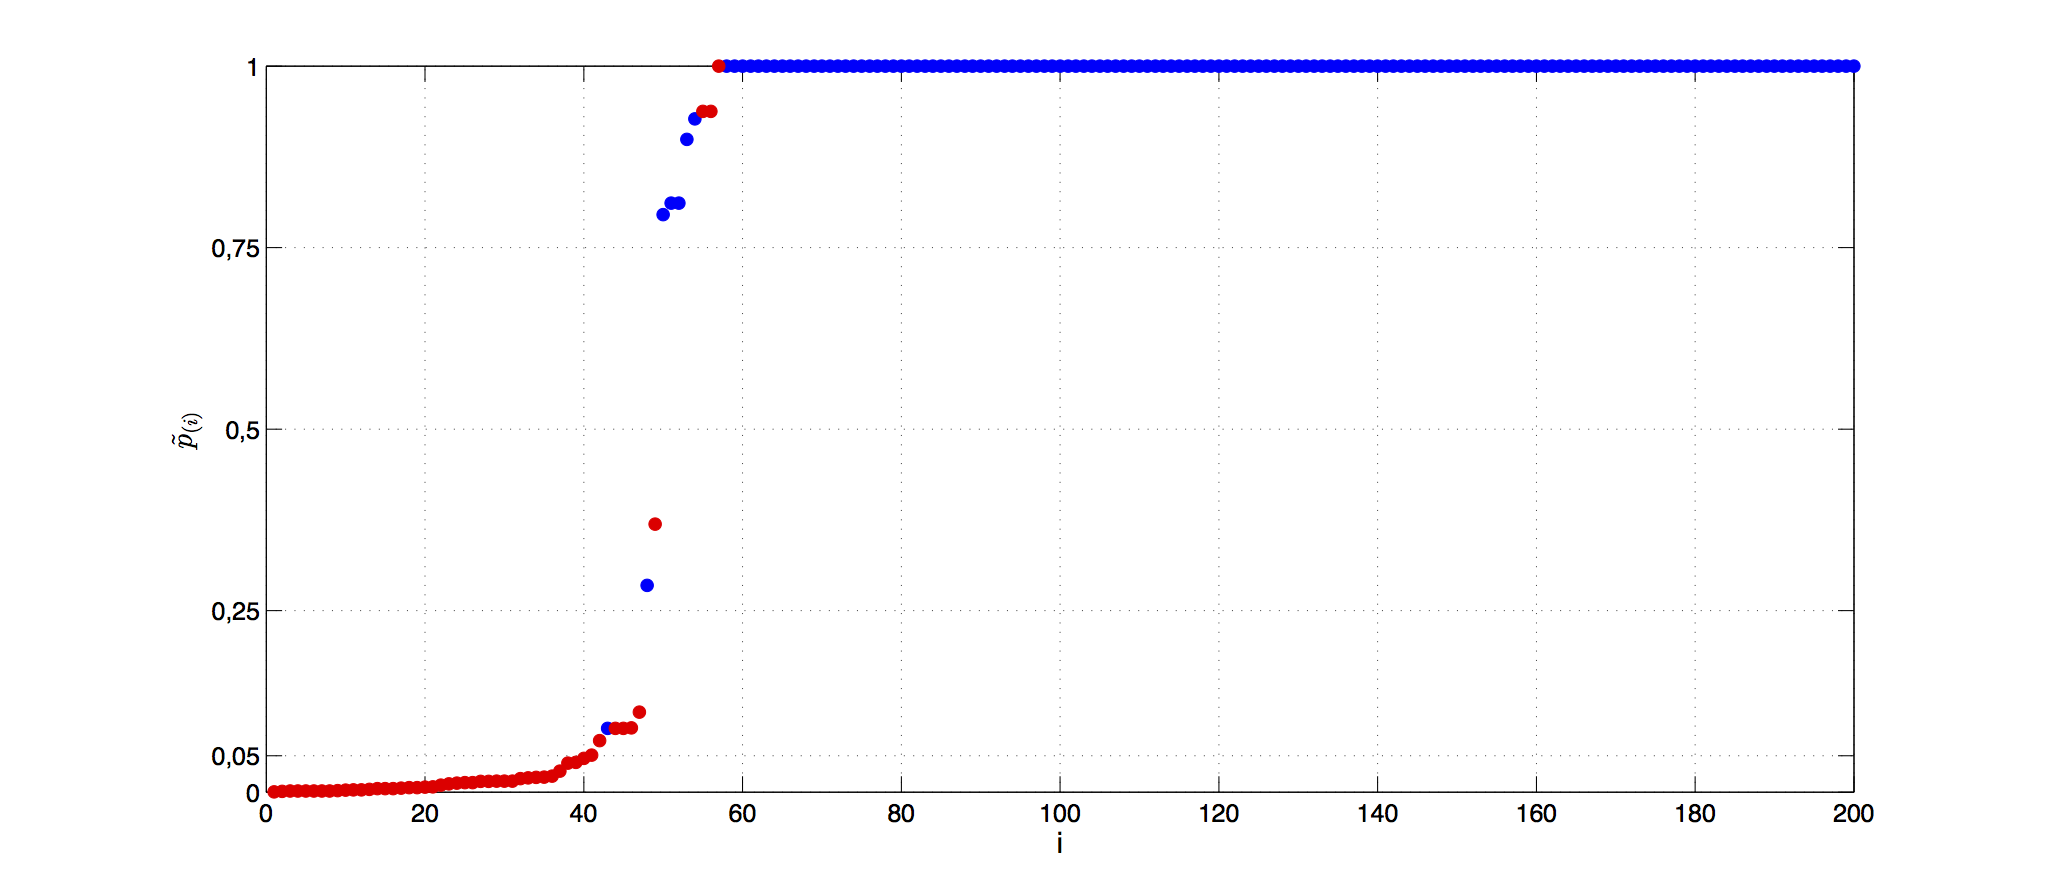
\includegraphics[width=0.8\textwidth]{ps_adj_by.png}
    \end{center}

    \begin{center}
        \begin{tabular}{ |r | c | c | c |}
        \hline
                          & Верных $H_i$ & Неверных $H_i$ & Всего \\ \hline
        Принятых $H_i$    & 150          & 10             & 160   \\ \hline
        Отвергнутых $H_i$ & 0            & 40             & 40    \\ \hline
        Всего             & 150          & 50             & 200   \\ \hline
        \end{tabular}
    \end{center}
    }
\end{frame}


\section{Примеры задач}
\subsection{}
\begin{frame}{Мутации}
%%%%%%%%%%%%%%%%%%%%%%%%%%%%%%%%%%%%%%%%%%%%%%%%%%%%%%%%%%%%%%%%%%%%%%%
% давайте рассмотрим гипотетический пример. Пусть есть 100 больных людей и 100 здоровых, и хочется понять, есть ли связь между болезнью и какой-то мутацией. В контрольной выборке из 100 человек мутация есть у одного, а в выборке больных — у 8 (таблица 9.9). По всей видимости, эта мутация достаточно редкая. Если сравнить доли людей с мутацией в выборках больных и здоровых, получится достигаемый уровень значимости p = 0.03, и гипотеза об отсутствии связи между мутацией и болезнью отвергается.
% Пусть теперь выдвигается еще одна гипотеза: наличие заболевания связано с тем, с гласной или согласной буквы у пациентов начинаются фамилии. В контрольной выборке здоровых людей у 36 человек фамилия начинается с гласной буквы, а в выборке больных — у 40 из 100 (таблица 9.9). При сравнении этих долей биномиальным критерием получается достигаемый уровень значимости 0.66, гипотеза отклонена не будет. Проблема, однако, заключается в том, что теперь в исследовании проверяются две гипотезы, и необходимо делать поправку на множественность этой проверки.
% Какой бы при этом ни использовался метод поправки, будь то метод Бонферрони, Холма или Бенджамини Хохберга, самый маленький достигаемый уровень значимости во всех них сравнивается с альфа/m . Таким образом, если требуется обеспечить контроль над какой-то мерой числа ошибок первого рода на уровне 0.05, нужно сравнивать самое маленькое значение достигаемого уровня значимости с 0.025. Самый маленький достига- емый уровень значимости в этом исследовании p = 0.03. Получается, эта нелепая гипотеза, которая была введена в исследование, замаскировала, возможно, неверную нулевую гипотезу, связанную с мутацией.
% Отсюда вытекает рецепт лучшего способа борьбы с эффектом множественной проверки гипотез: проверять меньше гипотез. Необходимо до начала исследования подумать, какие из возможных гипотез на самом деле не представляют интереса, и отказаться от их рассмотрения. За счет этого появится возможность сделать более либеральную поправку на множественность и отвергнуть больше действительно неверных гипотез, совершить больше действительно интересных открытий. Важно, что такая фильтрация гипотез должна осуществляться именно до сбора данных. Если выбрасывать гипотезы уже после того, как стали известны достигаемые уровни значимости, возникнет эффект переобучения.
%%%%%%%%%%%%%%%%%%%%%%%%%%%%%%%%%%%%%%%%%%%%%%%%%%%%%%%%%%%%%%%%%%%%%%%
    \begin{center}
    \begin{tabular}[t]{|m{3cm}|c|c|c|}
        \hline
                                     & Контроль (100) & Больные (100) & $p$ \\ \hline
        Мутация                      & 1 из 100       & 8 из 100      & 0.0349 \\\hline
        Фамилия начинается с гласной & 36 из 100      & 40 из 100     & 0.6622 \\\hline
    \end{tabular}
    \end{center}

    \bigskip

    Бонферрони, Холм: $p_1$ сравнивается с $\frac{0.05}{2}=0.025$

    Шидак: $p_1$ сравнивается с $1-\left(1-0.05\right)^{\frac1{2}}\approx0.02532$
\end{frame}

\begin{frame}{Подгруппы}
    \only<1>{
%%%%%%%%%%%%%%%%%%%%%%%%%%%%%%%%%%%%%%%%%%%%%%%%%%%%%%%%%%%%%%%%%%%%%%%
% Эффект множественной проверки гипотез ярко проявляется при анализе подгрупп. Для примера можно рас- смотреть следующее исследование, в котором принимают участие 1073 пациента с ишемической болезнью сердца1. Их делят на 2 подгруппы (в зависимости от типа лечения) и исследуют взаимосвязь между выжи- ваемостью и типом лечения. Требуется понять, какой их двух типов лечения лучше.
% Важные факторы, которые влияют на выживаемость при ишемической болезни сердца, — это число пора- женных артерий, (может быть 1, 2 или 3), и тип сокращений левого желудочка (нормальный и абнормальный). В таких ситуациях исследователи часто хотят посмотреть на сравнительную эффективность типов лечения отдельно во всех подгруппах по уровням важных факторов. В данном случае два фактора порождают 6 подгрупп, в каждой из них сравнивается выживаемость пациентов по двум типам лечения.
%%%%%%%%%%%%%%%%%%%%%%%%%%%%%%%%%%%%%%%%%%%%%%%%%%%%%%%%%%%%%%%%%%%%%%%
    (Lee et al., 1980): 1073~пациента с~ишемической болезнью сердца были искусственно разделены на две случайные группы, лечение в двух группах проходило одинаково. 
    Исследовалась выживаемость пациентов.

    \bigskip

    Важными факторами, влияющими на выживаемость, являются число поражённых артерий (одна, две, три) и тип сокращений левого желудочка (нормальный, абнормальный).

    Для одной из шести подгрупп по этим уровням фактора были обнаружены значимые различия в выживаемости пациентов первого и второго типов.
    }

    \only<2>{
%%%%%%%%%%%%%%%%%%%%%%%%%%%%%%%%%%%%%%%%%%%%%%%%%%%%%%%%%%%%%%%%%%%%%%%
%В одной из 6 подгрупп были обнаружены значимые различия в выживаемости пациентов при лечении первого типа и второго. На рисунке показаны кривые выживаемости пациентов этих подгрупп. По ним видно, что в группе лечения A после 6 лет наблюдений выжило меньше 40% пациентов, а в группе, соответствующей лечению B, — в районе 60\%. Это различие статистически значимо. Кажется, что для пациентов с таким числом пораженных артерий и с таким типом сокращения левого желудочка лечение B действительно существенно эффективнее.
% На самом деле эти два лечения отличаются только названием, и две группы пациентов лечились абсолютно одинаково. Эта статья была написана с целью показать необходимость поправки на множественную проверку гипотез при анализе подгрупп. Действительно, при сравнении кривых выживаемости во всех 6 подгруппах, проверяются 6 абсолютно независимых гипотез, и возникает эффект множественной проверки. Если подгрупп достаточно много, в результате будут всегда получаться какие-то значимые отклонения.
%%%%%%%%%%%%%%%%%%%%%%%%%%%%%%%%%%%%%%%%%%%%%%%%%%%%%%%%%%%%%%%%%%%%%%%
    \begin{center}
        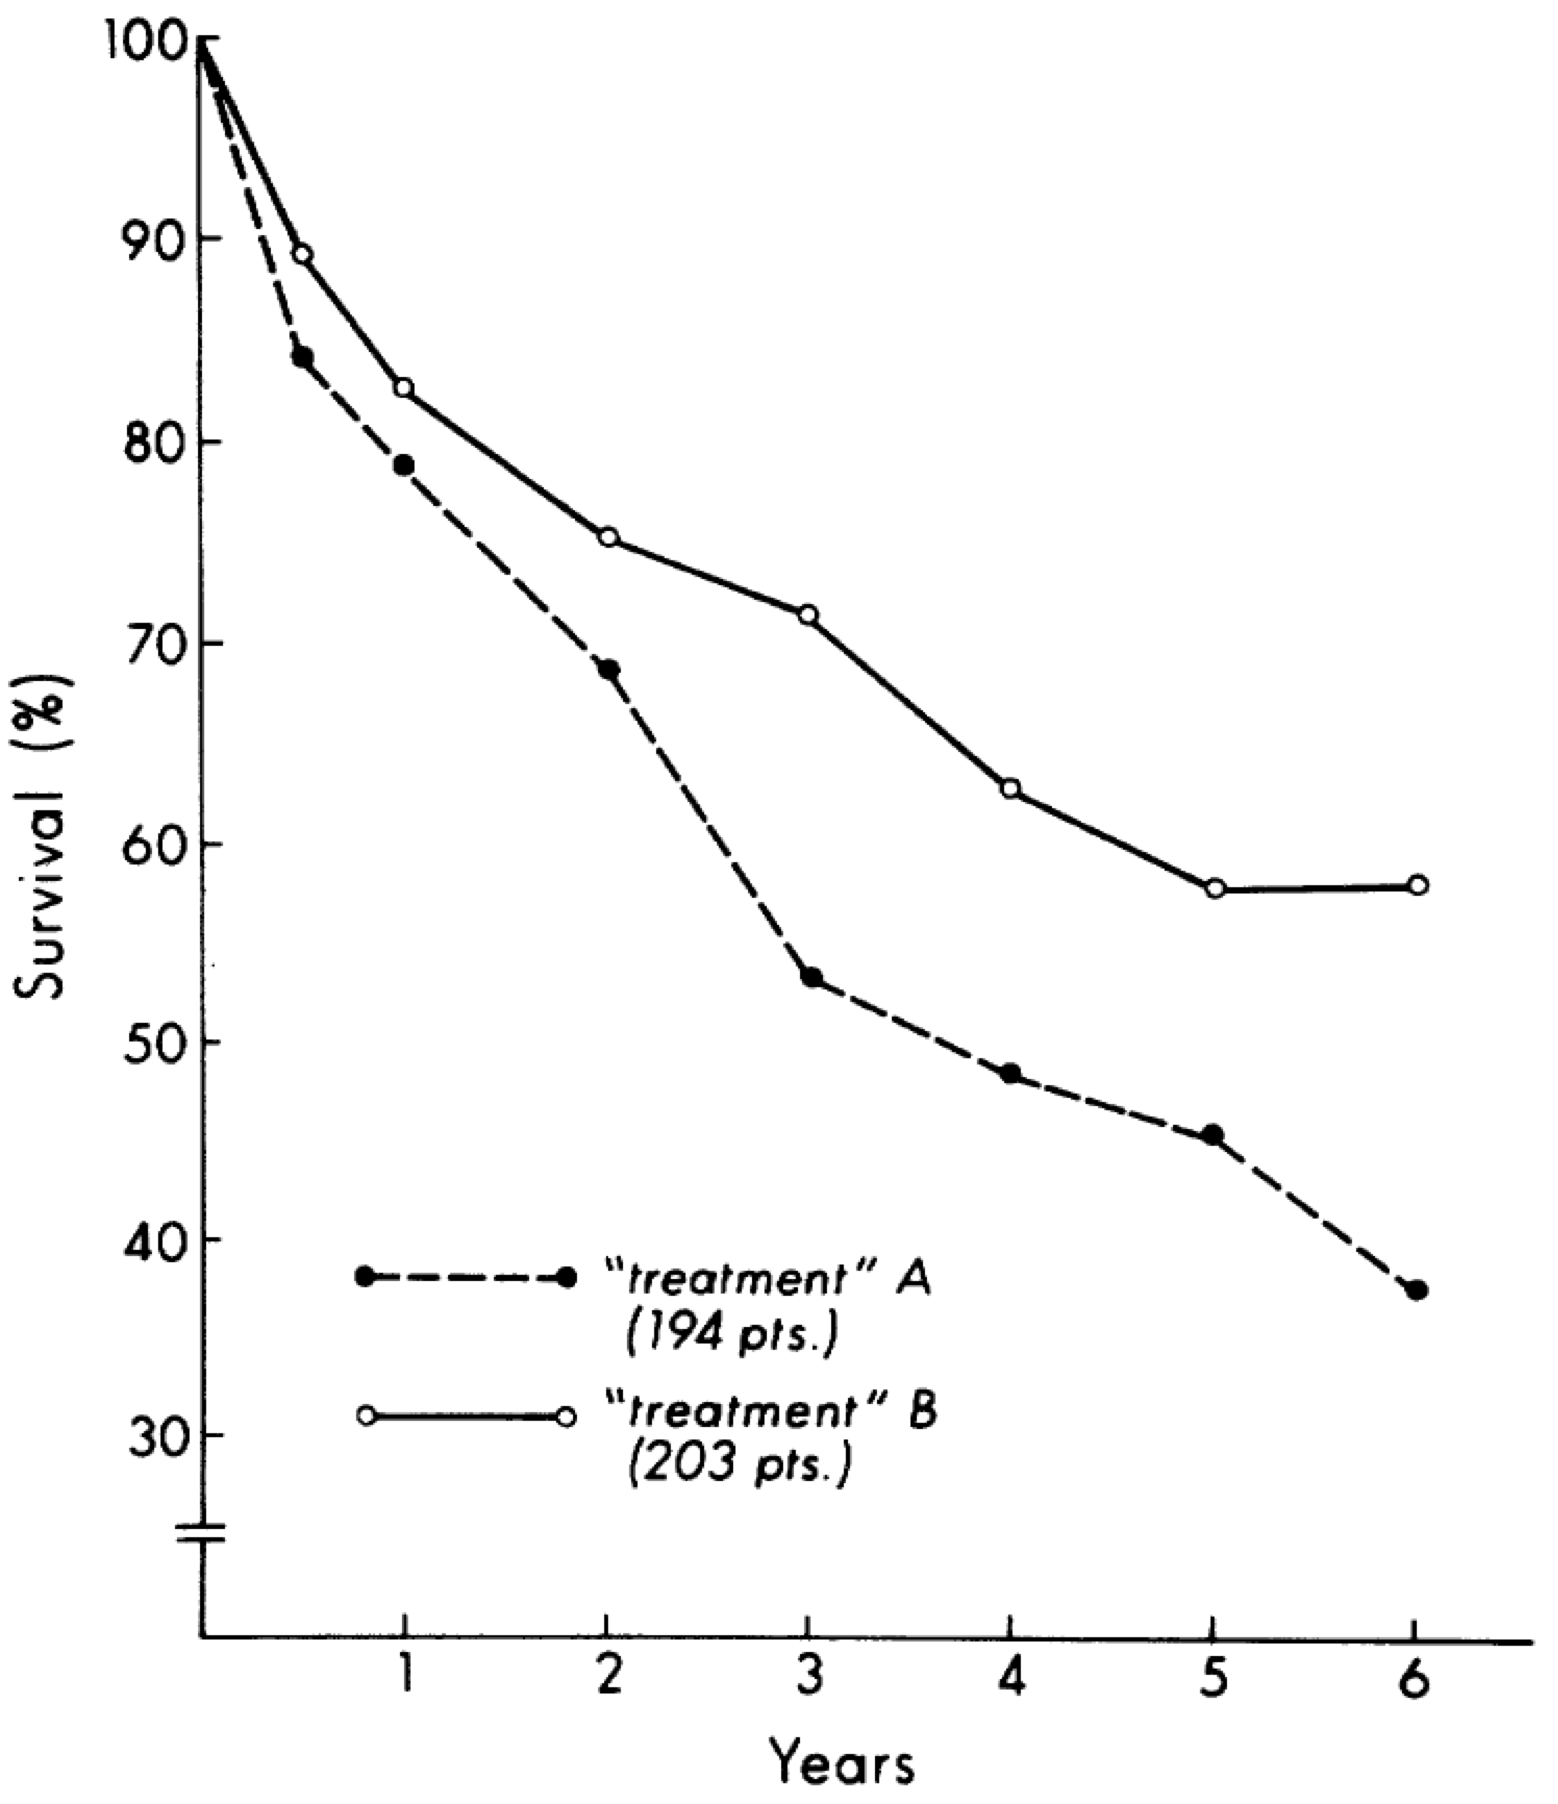
\includegraphics[height=0.75\textheight]{surv.png}
    \end{center}
    }

    \only<3>{
%%%%%%%%%%%%%%%%%%%%%%%%%%%%%%%%%%%%%%%%%%%%%%%%%%%%%%%%%%%%%%%%%%%%%%%
%Eсть и исследование, в котором такая ошибка в анализе подгрупп была совершена на самом деле, — это исследование 2008 года, в котором изучалась связь между употреблением кофеина и риском возникновения рака груди. В этой статье всего было около 50 разных подгрупп, по самым разным уровням различных факторов. В частности, было показано, что употребление более чем четырех чашек кофе в день связано с увеличением риска злокачественного рака груди (достигаемый уровень значимости p = 0.08). Это больше, чем стандартный уровень значимости 0.05, но меньше чем либеральный уровень значимости 0.1. Кроме того, потребление кофеина свя- зано с увеличением риска возникновения эстроген- и прогестерон- независимых опухолей, а также опухолей размером больше 2 сантиметров (достигаемый уровень значимости p = 0.02). Еще одно открытие: потребление кофе без кофеина связано со снижением риска возникновения рака груди у женщин в постменопаузе, принимающих гормоны (достигаемый уровень значимости p = 0.02).
% Ясно, что за счет большого количества рассматриваемых подгрупп можно всегда получить какие-то значи- мые отклонения, если не делать поправку на множественную проверку. Какие-то из этих открытий с большой вероятностью окажутся ложными. В каком-то смысле это напоминает переобучение: оценивается эффектив- ность лечения в разных подгруппах в зависимости от каких-то признаков пациента, и если эти признаки слишком сложные и их слишком большое количество, то происходит переобучение под анализируемую вы- борку. В качестве экстремального примера такого переобучения можно вспомнить цитату из Галена, II века до нашей эры: «Все больные, принявшие это средство, вскоре выздоровели, за исключением тех, кому оно не помогло — они умерли. Отсюда очевидно, что средство помогает во всех случаях, кроме безнадежных».
%%%%%%%%%%%%%%%%%%%%%%%%%%%%%%%%%%%%%%%%%%%%%%%%%%%%%%%%%%%%%%%%%%%%%%%
    (Ishitani, Lin, 2008): анализировалась связь потребления кофеина, кофе и~чая и риска возникновения рака груди, всего около 50~подгрупп. Показано, что:
    \begin{itemize}
    \item употребление четырёх и более чашек кофе в день связано с~увеличением риска злокачественного рака груди ($p=0.08$);
    \item потребление кофеина связано с увеличением риска возникновения эстроген- и прогестерон-независимых опухолей и опухолей больше 2~см ($p=0.02$ и $p=0.02$);
    \item потребление кофе без кофеина связано со снижением риска рака груди у женщин в постменопаузе, принимающих гормоны ($p=0.02$).
    \end{itemize}

    \bigskip

    См. также:
    \begin{itemize}
	    \item (Гален, II~в. н.э.): "Все больные, принявшие это средство, вскоре выздоровели, за~исключением тех, кому оно не помогло — они умерли. Отсюда очевидно, что это средство помогает во всех случаях, кроме безнадежных." 
        \item \url{http://youtu.be/QysrgLXMPwA}
        \item \url{http://xkcd.com/882/}
        \item \url{http://wmbriggs.com/blog/?p=9308}
    \end{itemize}
    }
\end{frame}

\begin{frame}{Cherry-picking}
%%%%%%%%%%%%%%%%%%%%%%%%%%%%%%%%%%%%%%%%%%%%%%%%%%%%%%%%%%%%%%%%%%%%%%%
% Другой интересный подход к множественной проверке гипотез называется cherry-picking. Обычно, когда вы проверяете много гипотез, вы заранее выбираете какую-то меру числа ошибок первого рода (например, FDR), и процедура, её контролирующая, говорит, что обеспечивая FDR<0.05, вы можете отвергнуть такие-то гипотезы из проверяемых. Cherry picking позволяет действовать наоборот: независимо от того, какие p-value вы получили, вы можете выбрать любое множество гипотез, которые вы хотите отвергнуть, а процедура автоматически даст верхнюю оценку доли ложно отклоняемых среди этих гипотез - и это именно доля, FDP - false discovery proportion, а не её матожидание, как у методов Бенджамини. Такой подход удобен в задачах, когда есть большое количество дополнительной информации о проверяемых гипотезах. Например, представьте, что вы проверяете наличие связи между наличием разных мутаций и каким-то заболеванием. На выходе вам нужно получить список мутаций, потенциально связанных с этим заболеванием, для последующей перепроверки. Всего разным мутаций мошут быть сотни тысяч, поэтому контролировать FWER в этой задаче не вариант - вы просто ничего не отвергнете, скорее всего. Кроме того, из предыдущих исследований, о которых вы читали в статьях, вы можете что-то знать про интересные гены, в которых мутации потенциально связаны с этим заболеванием. Вы можете расчитать составить ваш финальный список, взяв за основу мутации, у которых получился очень маленький p-value, и убрав и добавив к нему какие-то другие по экспертным соображениям. Если процедура говорит, что в таком списке доля ложных гипотез невелика, значит, это хороший список.
%%%%%%%%%%%%%%%%%%%%%%%%%%%%%%%%%%%%%%%%%%%%%%%%%%%%%%%%%%%%%%%%%%%%%%%
	Метод cherry-picking:
	\begin{itemize}
		\item выбираем произвольное множество $\mathbf{R}$ гипотез, которые мы хотим отвергнуть;
		\item оцениваем сверху долю ложных отклонений: $$FDP=\frac{V}{R}.$$
	\end{itemize}
	
	Оценка справедлива сразу для всех $2^m-1$ возможных множеств $\mathbf{R}$.
\end{frame}


\begin{frame}{Большая часть исследований неверна}
%%%%%%%%%%%%%%%%%%%%%%%%%%%%%%%%%%%%%%%%%%%%%%%%%%%%%%%%%%%%%%%%%%%%%%%
% Интересно, что эффект множественной проверки гипотез проявляется не только на уровне отдельных исследований, но и на уровне науки в целом. Например, существует большое количество научных групп, изучающих механизмы и причины возникновения рака, и, например, его связь с рационом. Даже если экспериментальные условия и определения во всех работах этих групп одинаковы, они неизбежно получают разные оценки эффекта употребления какого-то конкретного продукта на вероятность возникновения рака - просто из-за случайности выборок. В итоге мы получаем, что по разным данным употребление молока ассоциировано одновременно и с увеличением, и со снижением риска рака. Чтобы разрешить такие противоречия, проводят мета-анализ - совместный анализ всех опубликованных результатов по какой-то выбранной теме. Оценка размера какого-то эффекта, сделанная по данным всех экспериментов сразу, гораздо более устойчива.
%%%%%%%%%%%%%%%%%%%%%%%%%%%%%%%%%%%%%%%%%%%%%%%%%%%%%%%%%%%%%%%%%%%%%%%
    \begin{figure}
    	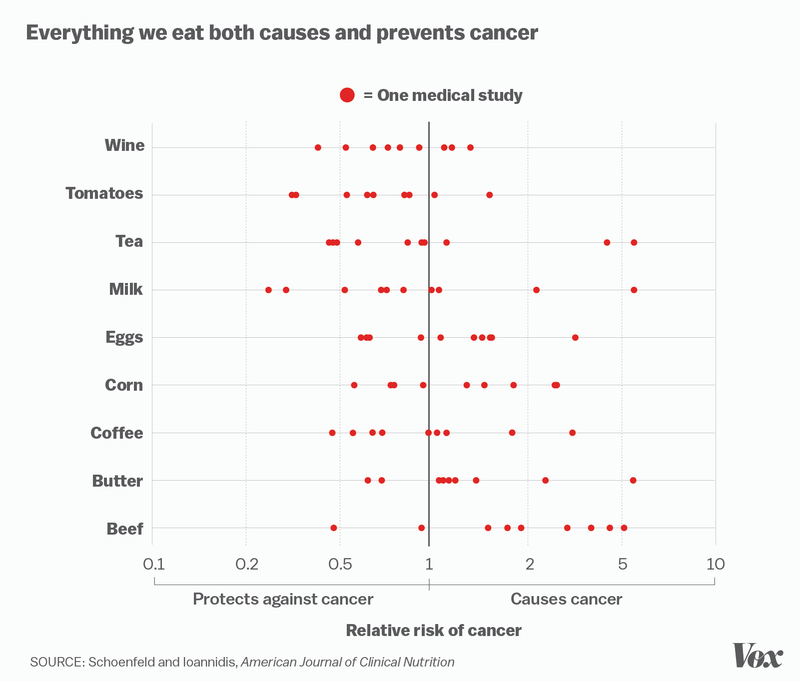
\includegraphics[width=0.55\textwidth]{Medical_studies.png}
    \end{figure}
	
	Ioannidis, Why most published research findings are false, 2005.
\end{frame}


%\begin{frame}{Примеры}
%	Сравнение качества модификаций алгоритма С4.5:
%	
%	\url{https://yadi.sk/d/KY2TqTuZeuxM9}
%	
%	\bigskip
%	
%	Транскриптом лейкоцитов детей, больных астмой (для самостоятельной работы):
%	
%	\url{http://www.ncbi.nlm.nih.gov/sites/GDSbrowser?acc=GDS4896}
%	\url{https://yadi.sk/i/av5eYc9teuxMd}
%\end{frame}

\section{}
\begin{frame}
    \frametitle{Литература}
\only<1>{    
    \begin{itemize}
    \item попроще~--- Bretz, посложнее~--- Dickhaus, хороший краткий обзор~--- Goeman, 2014;
    \item перестановочные методы (permutation methods)~--- Westfall, 2008, и~другие работы этого автора;
%    \item positive orthant dependence~--- Holland, 1987;
%    \item subset pivotality~--- Westfall, 2008;
%    \item PRDS~--- Benjamini, 2001;
	\item cherry-picking~--- Goeman, 2011;
    \item случайные поля~--- Nichols, 2003; \url{fil.ion.ucl.ac.uk/spm/}, \url{coursera.org/course/fmri}.
    \end{itemize}

    \bigskip

    {\small
    Bretz F., Hothorn T., Westfall P. \textit{Multiple Comparisons Using R}, 2010.
		
		\vspace{5pt}
		    	
    Dickhaus T. \textit{Simultaneous Statistical Inference With Applications in the Life Sciences}, 2014.
		
		\vspace{5pt}
		
	Goeman J.J., Solari A. (2011). \textit{Multiple testing for exploratory research}. Statistical Science, 26(4), 584–597. 
		
		\vspace{5pt}
				
	Goeman J.J., Solari A. (2014). \textit{Multiple hypothesis testing in genomics}. Statistics in Medicine, 33(11), 1946–1978. 
		
		\vspace{5pt}
		
    Ioannidis J.P.A. (2005). \textit{Why most published research findings are false}. PLoS Medicine, 2(8), e124. 
	}
	}
	\only<2>{\small
	Ishitani K., Lin J. (2008). \textit{Caffeine consumption and the risk of breast cancer in a large prospective cohort of women}. Archives of Internal Medicine, 168(18), 2022–2031. 	
		
		\vspace{5pt}
			
	Lee K.L., McNeer J.F., Starmer C.F., Harris P.J., Rosati R.A. (1980). \textit{Clinical judgment and statistics. Lessons from a simulated randomized trial in coronary artery disease}. Circulation, 61(3), 508–515. 
		
		\vspace{5pt}
		    			    	
    Nichols T.E., Hayasaka, S. (2003). \textit{Controlling the familywise error rate in functional neuroimaging: a comparative review}. Statistical Methods in Medical Research, 12(5), 419–446.
		
		\vspace{5pt}
		    			    	
    Westfall P., Troendle J. (2008). \textit{Multiple testing with minimal assumptions}. Biometrical Journal, 50(5), 745–755.

%    Holland B.S., Copenhaver M.D. (1987). \textit{An Improved Sequentially Rejective Bonferroni Test Procedure}. Biometrics, 43(2), 417–423.

%    Benjamini Y., Yekutieli D. (2001). \textit{The control of the false discovery rate in multiple testing under dependency}. Annals of Statistics, 29(4), 1165–1188.
	}
\end{frame}

\begin{frame}{Проверка симметрии}

\begin{itemize}
\item В основном проверка идет при знании центра распределения
\begin{itemize}
    \item Критерий Вилкоксона
    \item Критерий Смирнова
\end{itemize}
\item Критерии, с эмпирической оценкой центра и дальнейшим тестом симметричности
\begin{itemize}
    \item Бхатачарья-Гаствирта-Райта (модифицированный Вилкоксон)\\
    $y_i = x_{[nq + 1]} - x_{[nq + 1 - i]},  z_i = x_{[N - nq + i]} - x_{[N - nq]}$
    \item Критерий Бооса 
\end{itemize}
\item Критерии проверки коэффициента ассиметрии
\item Подробнее, смотри учебник Кобзаря
\end{itemize}
\end{frame}


\begin{frame}{Проверочная работа}
\textbf{Формат:} несколько типовых задач из лекций 1--4.\\

\textbf{Длительность:} 20--30 минут.\\

\textbf{Когда:} 9 марта после семинара.\end{frame}

\end{document}
